% Allow relative paths in included subfiles that are compiled separately
% See https://tex.stackexchange.com/questions/153312/

\providecommand{\main}{..}
\documentclass[\main/thesis.tex]{subfiles}

\onlyinsubfile{\zexternaldocument*{\main/tex/introduction}}

\begin{document}

\chapter{Implementation}

% \section{Approach}
% \subsection{ANN approaches}
% Numerous deep, neural network models have been proposed and utilized for the purpose of signal generation in recent years. WaveGans and WaveNet have been subject to significant improvements and experiments since their proposal \cite{nsynth2017,yamamoto2020parallel,oord2017parallel}. Even more recently Variational AutoEncoders (VAE's) have been utilized for generation of short percussive samples \cite{aouameur2019neural,ramires2019timbfeat}. In this work however, we opt to use digital signal processing methods to create a virtual synthesizer for the generation of audio signals as it provides several unique advantages:
% \begin{enumerate}[label=\roman*]
%   \item Fast, offline rendering of audio with no reliance on GPU: Currently not possible with state of the art models such as parallel WaveGan \cite{yamamoto2019parallel} and parallel WaveNet \cite{oord2017parallel}. 
%   \item Rendering at high sampling rates: Performance speed being a common issue, the standard sampling rate in most audio generation work utilizing neural networks appears to be under 24 khz \cite{yamamoto2019parallel,oord2017parallel,aouameur2019neural,ramires2019timbfeat}. However, a significant number of untrained human ears can detect a change in quality of audio between sampling rates of 192 khz and the industry standard of 44.1 khz \cite{reiss2016meta} with a dramatic increase in quality detection after training. Therefore we can safely assume that most producers would prefer their audio samples to have sampling rates of 44.1 khz or higher. In this work, we fix our sampling rate to the 48 khz standard. 
%   \item Neural networks are viewed as unexplainable black box solutions \cite{basheer2000artificial}. Some models such as VAE's can learn an underlying latent space of parameters and capture the distinguishing features of the different labels in a dataset. However, these spaces are learned in an unsupervised manner and must be manually analysed, perhaps extensively, before they can be understood \cite{esling2018generative}. The use of a virtual synthesizer for audio generation makes our parameters readily understandable and easily modifiable. \\
% \end{enumerate}

% Automatic programming of virtual synthesizers has also been a topic of interest. In early 2000s, Interactive Genetic Algorithms (IGA's) were utilized for the generation of new sounds with various sound-engines \cite{johnson1999exploring,dahlstedt2001creating}. More recent work by Yee-King et al. \cite{yee2018automatic} used Long short-Term Memory (LSTM) models and genetic algorithms to find the exact parameters used to create a group of sounds. The sounds approximated were made by the same virtual synthesizer, not an external source; making the eventual replication certain even with random search. Since this work appears more focused on pads and textures rather than drums, feature matching appears to not be concerned with the envelope of the sounds but rather the frequency content within arbitrary time windows. Yet another recent, impressive work by Esling et al. used a large dataset of over 10,000 presets for a commercial VST synthesizer to learn a latent parameter space which can be sampled for creation of new audio \cite{esling2019universal}. As stated before, our work explores the rapid approximation of percussion sounds with no previous knowledge about the sonic capabilities of our virtual synthesizer, exploring the actual parameter space rather than its latent representation.
\label{impl}
\section{Our Goal}
Our goal is to create a system for the generation of novel drum sounds. In this chapter, we will discuss the two main components of our system: The \textit{virtual synthesizer} and the \textit{virtual ear}. A quick outline of our generative pipeline is this: Random programs will be sent to the virtual synthesizer, modifying its parameters. As the virtual synthesizer creates sounds based on these programs, the virtual ear will listen to the sounds and determine if they should be categorized as drums. If so, which category of drum do they belong to. 

Here we discuss in more detail the implementations and interactions of these two components. Later on in the chapter, we will discuss our dataset and code which can be used for replication of our project. 
\section{Virtual Synthesizer}
\label{vs}
We require a synthesizer of sound which is capable of rapidly receiving programs and rendering the corresponding sound offline. These programs can be generated randomly by the synthesizer iteself or created externally by a person or algorithm.  We anticipate that any synthesizer with such capabilities can be integrated into our system; Here, we do not prioritize perfect replication of organic sounds as unusual synthesis methods will likely lead to novel sound generation. As discussed in section~\ref{sec_digital_synthesis}, we opted for a set of classical DSP methods to build our synthesizer. For our project, we used the python based Pippi library for sound generation\footnote{https://github.com/luvsound/pippi}. This library uses a C back-end\footnote{https://github.com/PaulBatchelor/Soundpipe} and focuses on fast offline generation of audio signals.

% todo-add figure of how it would work
% AH-are they only sequentially composed?
Our virtual synthesizer contains a set of one or more submodules. Each submodule is a self-contained noise making unit. Submodules have identical sets of parameters, but widely different outputs can be achieved depending on the values assigned. The set of parameters available to each submodule is highlighted in Table~\ref{table:submodule_params}. The sonic output of the virtual synthesizer is the normalized addition of the sonic output of its submodules. Our implementation of a synthesizer can have any number of submodules. The parameters that dictate the output signal of each submodule as well as the range of values each parameter can take are shown in table~\ref{table:submodule_params}. We call the number of submodules in each virtual synthesizer the \textit{stack size}. We call the sets of parameter values that characterize a synthesizer's submodules a \textit{program} (analogous to a preset for a VST).  

As we are interested in short, one-shot percussive sounds, each virtual synthesizer program will generate a 1 second piece of audio. This 1 second limit is over twice the length of the average one-shot drum sample within our database. Each submodule can make an audio signal with the length of 0.1-1 second, and play it at any point within the 1 second rendering time (but the entire sound must fit within the second, that is, a 0.5 second sound cannot begin playing after 0.5 seconds within rendering time frame). If the synthesizer has a stack size of more than 1 the audio signals from each submodule are overlapped and the total amplitude is normalized.

The ADSR parameters shape the entire amplitude of the signal. Each submodule creates its signal at full amplitude then shapes it according to its internal ADSR parameter. Prior to being applied to the signal, each of these parameters is assigned an integer value in the range of 0-3, and normalized relative to the others such that \[ A_{norm} + D_{norm} + S_{norm} + R_{norm} = 1 \] \\ 
Where each value $v_{norm}$ in the $\{A_{norm}, D_{norm},S_{norm},R_{norm}\} $ set is normalized such that:
\begin{align*}
\text{for each $v$ $\epsilon$ \{A,D,S,R\}} \\
v_{norm} = \dfrac{v}{A + D + S + R}
\end{align*}
 The OSC type will determine the wave-shape of the signal. We limited this parameter to three fundamental wave forms: sine waves, square waves and saw waves. We also allow the creation of noise signals, which can imitate timbral characteristics of higher pitched drum samples at a very low computation cost (relative to the addition of thousands of sine waves at various frequencies). If the IsNoise boolean is set to true, the OSC type parameter loses importance as the OSC type will simply be used for the generation of noise via random wavetable transformations. Before the filter and ADSR envelope take affect, the generated noise will have similar characteristics to white noise. 

Each submodule is a monophonic synthesizer. That is, each submodule can play one note (or frequency) at a time. However, quick changes in pitch can occur in drum sound. Our more successful attempts at creation of synthetic kick or bass drums are often characterized by quick, exponential decrease of a sine-wave's pitch from medium to low audible frequencies. To mimic such sounds, synthesizer submodules may slide between 4 different pitches in the 1 second time frame. Each pitch value is a midi note with a frequency and length value. Each submodule accepts a list of 5 consecutive possible pitch values. The submodule will play each note in the list consecutively after normalizing the length values. The pitch notes are played in a portmanteau fashion such that there is no audible gap. This normalization of length values is similar to that of the ADSR values. 

% Considering this setup, we predict that in order to generate kick drums using these parameters, the list of notes must vary from high frequencies to low; While other drum types such as hats or shakers require all pitch values to remain static, such that pitch bending does not occur. 



\begin{table}[h!]
\centering
\resizebox{\columnwidth}{!}{\begin{tabular}{ |c|c|c| } 
\hline
Parameters & Value Range & notes and constraints\\
\hline \hline
Attack & 0-3 & A-D-S-R values relative\\
Decay & 0-3 & relative to A-S-R\\
Sustain & 0-3 & relative to A-D-R\\
Release & 0-3 & relative to A-D-S\\
OSC type & sine,square,saw & tone type\\
IsNoise & boolean & whether to generate noise\\
Length & 0-1 second & - \\
StartTime & 0-1 second & Length+Start$<$1\\
Amplitude & 0.1-1 & 1 = max amplitude\\
Pitches(notes) & list of pitches &  range of C0(16.35hz) to B9 \\
HP filter Cuttoff & 0-20000hz & -\\
LP filter Cuttoff & 20000-HP & never lower than HP cutoff\\
Filter Order & 4,8,16 & butterworth filter order \\
\hline
\end{tabular}}
\caption{Synthesizer submodule Parameters. Despite the simplicity of the parameters and our efforts at constraining the ranges, the number of parameters that can be randomly chosen for each submodule is in the order of $10^{15}$ }
\label{table:submodule_params}
\end{table}


\section{The Ear}

What we refer to as an "ear" is any method of scoring and classifying audio (e.g machine listening) \cite{malkin2006machine,rowe1992interactive}; The ideal ear for our task will be capable of "listening" to a piece of audio and giving it a score (or a list of scores) based on how well it satisfies certain criteria. In this work we are mainly focused on percussive generation, therefore, what we require from the ear is to give us probabilities of an audio sample belonging to various categories. As our synthesizer outputs are close to deterministic for all programs, the evaluations of the ear would allow us to associate scores of the sound with the program that generated it. In section~\ref{gens} we discuss how these scores can be used to navigate synthesis towards parameters which give us the desired sonic output.

We are not looking for the perfect imitation of organic drums using a synthesizer. We seek to imitate drums using a synthesizer and even \textbf{prefer} for its generations to retain novel, unusual characteristics. The task assigned to the virtual ear is the rejection of "noise" from the virtual synthesizer and the rare acceptance of drum-like sounds. By definition, we cannot anticipate what these novel drums will sound like. Considering the limitations of learning by example, and since raw data can clearly separate organic drums from virtual synthetic noise, we believe that transformation and filtering of raw sound data is a critical step of the listening process; A step that will assist with the extraction of the fundamental characteristics that we are seeking and prevent the rejection of novel sounds.

 With our dataset of labeled drum sounds, discussed in~\ref{data}, we can confidently categorize unlabeled drum sounds given that we know they are drum sounds. However, a major hurdle towards the implementation of a \textquotedblleft drum from non-drum \textquotedblright recognizing ear is that the set of sounds that are not percussive is infinite. 

In our case, drum groups are an example of closed sets, since we believe that a sufficiently large sample pack can effectively describe common drum categories. However, effective representation of all possible non-drum sounds is not attainable via examples alone. We hypothesize that the implementation of our virtual ear falls outside the traditional categorization problem and within the "Open Set Recognition" (OSR) domain~\cite{geng2020recent,mundt2019open}. 

Traditional classification tasks often make the assumption the data points used for training the model and future unlabeled data will emerge from the same system of processes~\cite{geng2020recent,mundt2019open}. This assumptions requires that sufficient positive examples of all possible classes exist and are trained on. Works toward the implementations of GANs have documented scenarios in which networks will assign high categorization probabilities to nonsensical, out of context data which should be rejected rather than categorized~\cite{geng2020recent,mundt2019open,hassen2020learning}.  

Once a sound is generated and passed onto the ear, we expect the virtual ear to facilitate our actions in response to two important questions: 
\emph{
\begin{quote}
\text{Decision.1 Could the sound could be used as a drum?}\label{Decision.1}
\\
\text{Decision.2 If it does sound like a drum, what type of drum should it be?}\label{Decision.2}
\end{quote}
    }


\hypref{Decision.1} requires knowledge of what drums \textbf{do not} sound like, or knowledge of an infinitely large set, which cannot be fully represented via examples. Also a consideration is that the source of sounds used in training the model (organic drum sounds) will be fundamentally different from the source of unlabeled sounds we wish to categorize (noise from a synthesizer). Much easier to answer is \hypref{Decision.2}, where we found satisfying results with a variety of different approaches. We attribute the relative ease of \hypref{Decision.2} relative to~\hypref{Decision.1} to be reflective of the OSR problem. 



As our synthesizer rapidly produces sounds, the virtual ear will listen to the sounds and accepts those that satisfy some fundamental characteristics of drums. How we characterize this description is critical as it allows novel sounds to be accepted as part of the drum group despite their anomalies. We approached this problem by the implementation of various feature extraction methods as well as various models which use these features towards a solution for ~\hypref{Decision.2} and~\hypref{Decision.1}.

We cover the implementation of these virtual ear models in two sections: \emph{two phased ears} (TPEs) and \emph{embedding ears} (EEs). As we will discuss in the next sections, TPEs are a combination different models for each of ~\hypref{Decision.2} and~\hypref{Decision.1}; With the features utilized by these models being manually defined. EEs use a highly compressed, automatically encoded representation of sound to give simultaneous answers to both questions.

\subsection{Two Phased Ears}
\label{sec:ear}
\subsubsection{Feature Extraction}



% AH: you should make it 1 instance of a generated synth 
We only consider 1 second long sounds made with a single stacked synth, yet the set of possible synthesizer parameters (and we assume, the sound generated by the synth given these parameters) is extremely large. In our case, as discussed in Section ~\ref{survey}, the majority of sounds generated by the synth do not resemble percussion.  We determined that there are 2 steps necessary to effectively extract percussive sounds
from the randomly generated sounds produced by virtual synthesizers: 
\begin{enumerate}
   \item  Phase $1$: Binary separation of sounds with percussive features from non-percussive sounds.
   \item Phase $2$: Given confidence that the sound being categorized is percussive, categorizing its type.
\end{enumerate}
We are interested in extracting generalizable, domain agnostic features. In this work we rely entirely on Fast Fourier Transform (FFT) and by extension Short-time Fourier Transforms (STFT) for feature extraction. Using FFT, a signal can be represented by a vector with each index corresponding to a frequency-bin (a range of frequencies too close to be distinguishable) and the value at each index corresponding to the combined-magnitude of the frequencies within the bin. STFT can be employed when a more accurate representation is desired; via the application of the FFT to a sliding time-window on the signal to create a matrix (a list of vectors). This matrix can effectively represent the frequencies present in the signal at each time step, given the right window-length and hop-size (how much the window is shifted at each time-step).
\begin{figure}
\centering
\textbf{Visual Representation of Raw Features}\par\medskip
    \subcaptionbox{Recorded hat sample}{    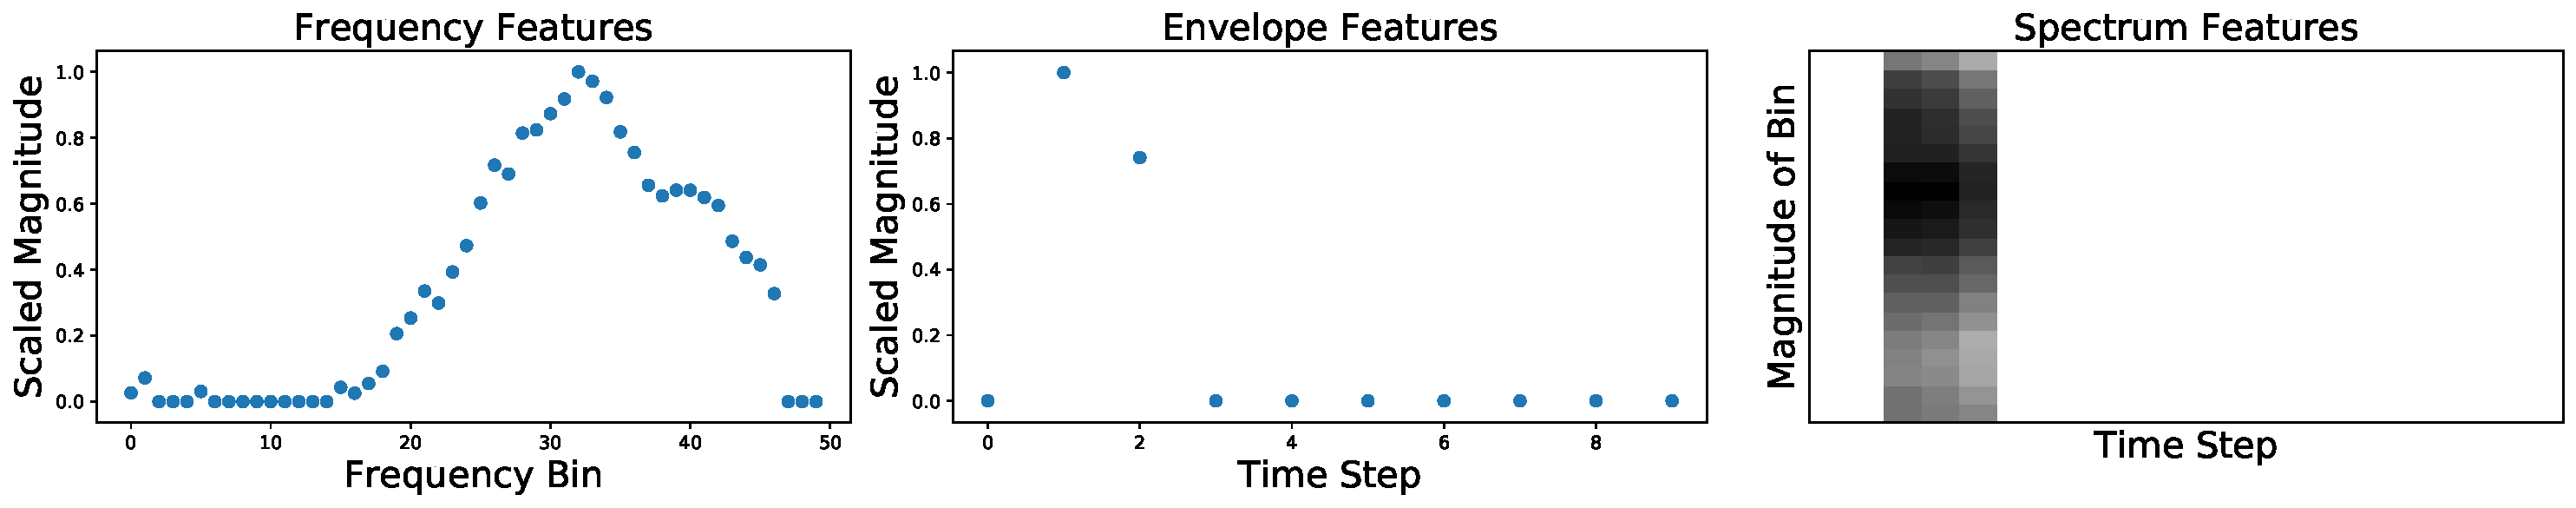
\includegraphics[width=1\columnwidth]{images/ff1.pdf}
    }
    \subcaptionbox{Randomly generated audio with percussive qualities, resembling a tight snare}{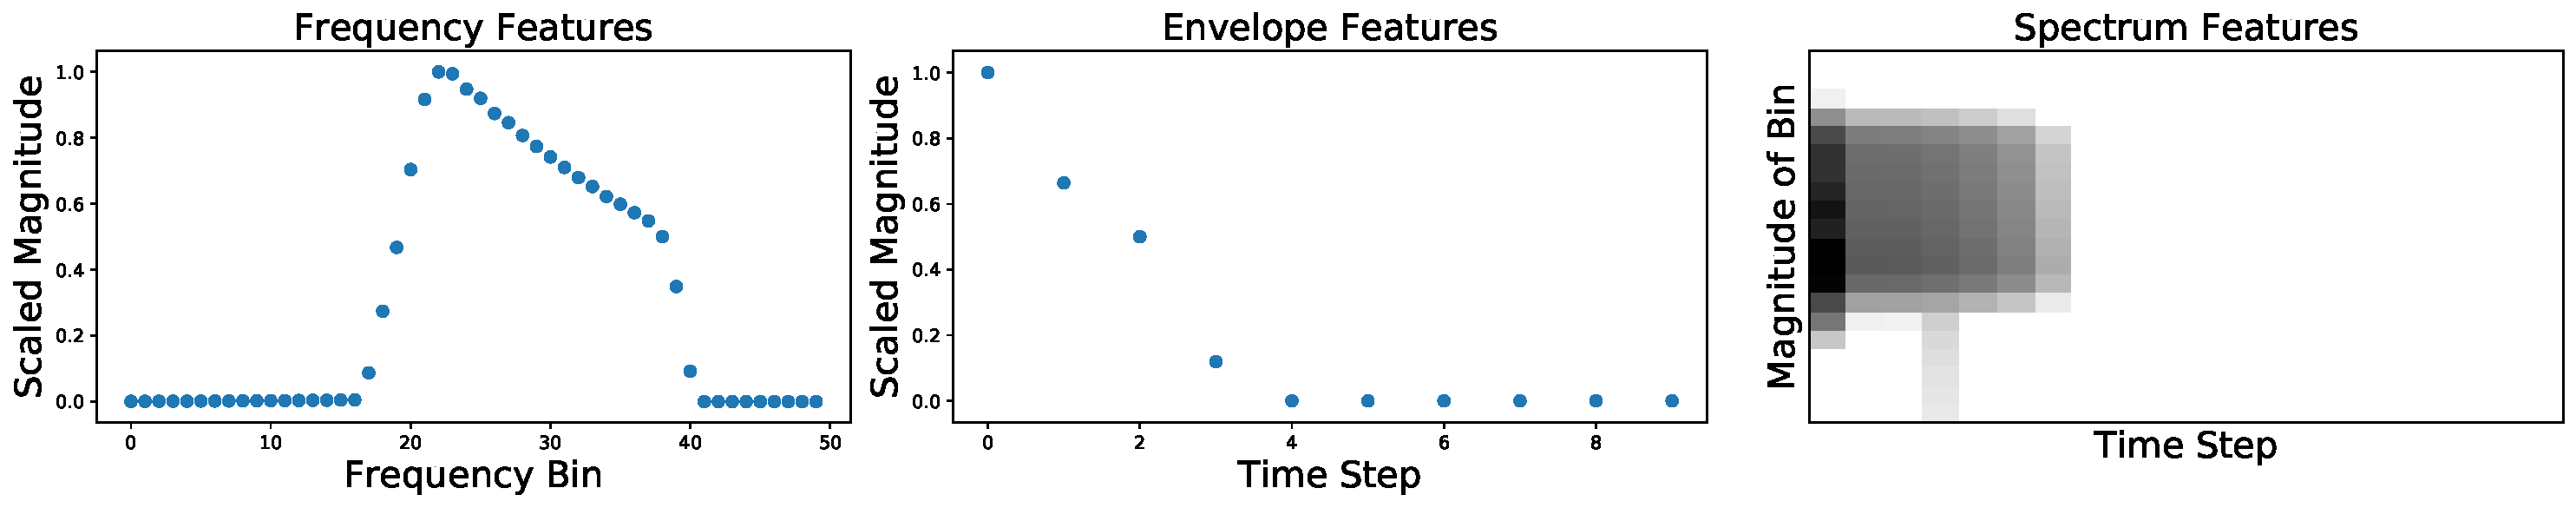
\includegraphics[width=1\columnwidth]{images/ff2.pdf}}
    \subcaptionbox{A randomly generated noise with a percussive envelop but non-percussive frequency features (modulated pitch)}
    { 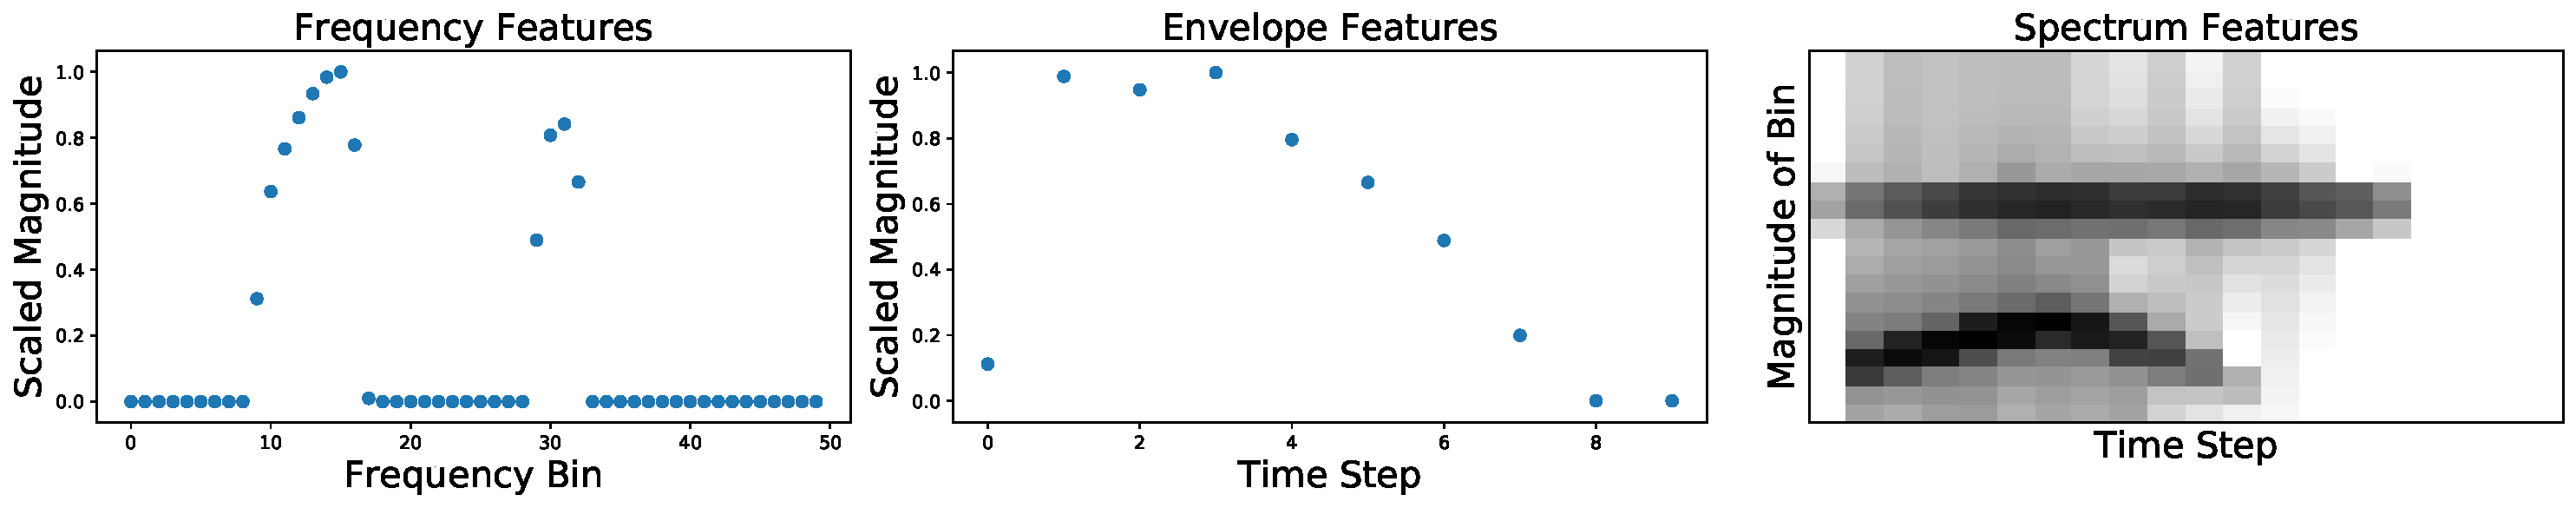
\includegraphics[width=1\columnwidth]{images/ff3.pdf}}
\caption{Graphed representation of features extracted for 3 different samples. Sample $a$ is a recorded hat from our database. sample $b$ is an example of randomly generated noise with percussive qualities that we found suitably similar to a snare sound. Sample $c$ is an example of a randomly generated noise where the spectrum features are necessary for proper classification.}
\label{fig:stackspectrums}
\end{figure}
% AH: If you need space shorten this paragraph to we use STFT which has worked in past and we use spectral-centroids and zero-crossings
Various works have demonstrated effective reconstruction of signals given their STFT~\cite{nawab1983signal,griffin1984signal}. For our purpose, if the original signal can be faithfully reconstructed from its STFT, analysis of the STFT may be relied on as source of fundamental features necessary for audible signal categorization. In the interest of keeping the feature space small and fundamental, other methods of feature extraction such as Spectral-Centroids~\cite{schubert2004spectral} and Zero-Crossing Rates~\cite{gouyon2000use} are not utilized.

Using only the STFT of signals as source of feature extraction we defined 3 transformation functions which we believe to capture important, unique attributes of percussive sounds.  These functions were applied at training time to 1 second audio samples before being sent to a classifier; transforming a signal into a set of features which we hope can capture the necessary information for our categorization task. 


\begin{enumerate}
\item Envelope Transformation: The goal of this feature is to capture the changes in loudness for the duration of the signal. Using STFT we generate a matrix $M_{i \times j}$ with rows $i$ and columns $j$ corresponding to time steps and frequency bins respectively, and with values $v_{i \times j}$ indicating the magnitude of the frequency bin $j$ at each time-step $i$. Information about the envelope of the signal can be extracted by summing the values of $M$ for each time-step (or row $i$), giving us a feature vector $v_i$. This vector is then normalized to the range of 0 to 1. The information contained in this vector is similar to that of a Root-Mean-Square measurement.
\item Frequency Transformation: A static, normalized snap-shot of the the frequencies present within the audio. The calculation of this feature vector is similar to the envelope, but the summation is done along the frequency axis. Another important distinction is that since capturing an adequate frequency resolution is important for this transformation, we utilized shorter hop-sizes and wider windows. A Mel Scale transformation was also applied in hopes that the captured features better represent human perception of frequencies. 
\item Spectrum Transformation: This function is simply a Mel Scaled STFT with its values normalized from 0-1. Since this features is a 2D matrix rather than a vector it captures more information about our signal but requires heavier, more complex computational methods to be utilized. 
\end{enumerate}

\subsubsection{The Models}
Using the described features, we trained several neural network models for Phase 1 and 2 in the Pytorch environment. The task of Phase 1 is to separate drums from not-drums (DrumVsNotDrum, or DVN). The task of Phase 2 is to categorize drums and percussion (DrumVsDrum, or DVD). We kept our feature space small, making it viable for feature selection and model design to be done on a trial and error basis. For all models, accuracy is calculated by prediction of all test dataset labels and the loss function and optimizer are Categorical-CrossEntropy and Adam respectively. Training continues until no reduction in loss and accuracy is observed in 10 epochs.  All activation functions are PReLU:
\begin {enumerate}
\item FC-DVN: Fully connected network trained on Envelope features, reaching 97\% accuracy on our test data for Phase 1. With size of 10x5x10.
\item CNNLSTM-DVN: A combination of CNN and LSTM models, where the CNN model extracts higher level features that are fed temporally to an LSTM cell. This model is trained on spectrum data and reaches 98\% accuracy on our test set. Its structure is the combination of a CNN with 2 output channels and kernel size $(7,3)$; Followed by an LSTM model of hidden size 800 and a fully connected layer of size 20x2.
\item E+F-DVD: A fully connected model trained on a concatenation of envelope and frequency features. Reaching 80\% accuracy for 6-way drum categorization in Phase 2. Size of 50x10x2x6.
\item CNN-DVD: A CNN model trained on Spectrum features. Reaching 82\% accuracy in a 6-way drum categorization in Phase 2. A combination of a CNN model with output channel size of 4, kernel of size of 5, another CNN model with output channel size of 8 and kernel of size 3. Followed by a fully connected network of shape 100x20x6.
\item FC-DVD: Fully connected 3 layer neural net with 78\% accuracy for 6-way drum categorization in Phase 2. Size of 400x200x50.
\end{enumerate}
The parameters are hand-picked and un-tuned. As discussed in section ~\ref{survey}, higher accuracy rates in these models do not translate to higher agreeableness with humans. leading us to believe that model accuracy on test data alone cannot be relied upon when the domain of sounds 
being categorized is switched from original percussion samples to virtual synth sounds.

With our models showing high accuracy on testing data, we combine models in order to increase the efficacy of each phase and address the "open set problem" for our task. For Phase 1 we only determine sounds as percussive if both FC-DVN and CNN-LSTM have determined it as such with over 90\% confidence. For the majority of our random generations that is not the case, but if a randomly generated sound has passed this phase, our three categorizers assign their categorizations to this sound. These categorizers have a moderate degree of agree-ability as seen in ~\ref{survey}, but often the decision is not unanimous. The fourth method of categorization, "averaged-cat", is implemented by taking the sum of the softmax outputs of all three categorizers, using it to determine the category. 

These models can be combined and weighted in various ways and the confidence thresholds can be modified in order to implement "virtual ears" with different properties. A glaring issue in the current implementation is the treatment of softmax outputs as a reasonable measure of a model's confidence. Ignoring that some models may have unwarranted higher confidence in their scores, skewing attempts at finding a consensus. 


\subsection{Embedding Ears}
% http://www.justinsalamon.com/uploads/4/3/9/4/4394963/cramer_looklistenlearnmore_icassp_2019.pdf says they need almost 40 million samples 
% http://www.cs.toronto.edu/~zemel/documents/prototypical_networks_nips_2017.pdf
% 
Like many other categorization tasks, we seek features that capture critical information about our data in the most compact format possible. In essence, feature extraction is often form of dimensionality reduction. While manual definition of the desired features can yield results, we also trained various autoencoder networks to encode our spectral features within small vectors. 

As discussed previously in section \ref{bg:NN}, many variations and applications of deep autoencoder networks have been proposed since Hinton et al. demonstrated effective dimensionality reduction via deep autoencoder networks \cite{hinton1994autoencoders,hinton2006reducing}. Particularly relevant are recent works by Aouameur et al. and Ramires et al. which influence the output of generative neural networks used for the synthesis of percussive sounds by inputting the low dimensional representation of desired traits \cite{aouameur2019neural,ramires2020neural}. 

As automatic encoding of short audio appears possible, we designed a number of autoencoder networks for the purpose of extracting features from our dataset of drum samples. Our designed networks are comprised of an encoder and a decoder. The encoder has the task of meaningfully projecting the spectrum data of each sound into a small bottleneck layer, while the decoder aims to use this projection to replicate the input data as closely as possible. Successful training will lead to an encoder network capable of projecting audio data into a low dimensional vector, in other words, a feature extractor. 

We kept our autoencoder designs relatively simple, all with approximately 150,000 parameters. Important to mention is that reported loss values of the model do not reflect whether the encoder will capture data that is useful for any purpose other than being utilized by the decoder. Also important is that we do not give any examples of synthetic noise to the encoders, and only train on organic drums. We hope that if a synthetic noise has drum-like characteristics, its compressed, latent representation given by the encoder will be similar to those of drum sounds and vice versa. We then use these latent expressions to train a support vector machine (SVM) model.
\begin{table}[h!]
\label{table:hyper_prams}
\begin{tabular}{|p{28mm}|p{50mm}|p{21mm}|p{21mm}|}
\hline
Hyper-Param. & Description  & Values & Distribution\\ \hline
Model Type      &   Affects encoder's first hidden layer & CNN,FC & Categorical \\  \hline
Optimizer       & Updates network's weights based on loss & Adam,SGD & Categorical  \\  \hline
Hidden Layers   & Extra hidden layer for the Encoder & True,False & Categorical \\  \hline
Time Steps & Temporal granularity of the spectrogram. Affects FFT windowing. & 10,20 & Categorical  \\ \hline
Learning Rate   &    Optimizer's learning rate  & $1^{-4}$ ... $1^{-1}$ & Uniform      \\ \hline
Frequency Bins & Number of spectrogram frequency bins & 10, 30,60 & Categorical \\ \hline

Regularization  &  L2 regularization parameter. Penalizes large weights to prevent overfitting & 1^{-6}~...~1^{-1} & Uniform\\ \hline
Latent Size & Size of bottle neck layer or number encoded features & 8,16,64 & Categorical              \\ \hline
Dropout Rate & Random zeroing of activations between layers to prevent over-fitting & 0,0.5,0.1 & Categorical\\  \hline
\end{tabular}
\caption{The Hyper-Paramter space in which the optimization was conducted.}
\end{table}
\subsubsection{Architecture and Hyper-Parameter Optimization}
% could do multi-objective pareto front stuff

Within the context of machine learning, a model's \emph{hyper-parameters} are fixed parameters which are set before the training begins (e.g number of layers, size of layers, loss function) and are not learned during the minimization procedure~\cite{bengio2000gradient}. Also within this context, hyper-parameter optimization is the task of searching for a set of hyper-parameters which would maximize the model's capacity, often done by a series of automatic test trials~\cite{bengio2000gradient,bergstra2011algorithms,bergstra2012random}. As a wide variety of viable autoencoder architectures have been proposed~\cite{aouameur2019neural,esling2018generative,gensler2016deep,zhang2016facing,pu2016variational}, we are faced with a number of choices for autoencoder design. To assist us with the construction of our model, we defined a number of possible choices for the architecture of our model and audio-transformers and used hyper-parameter optimization to extract promising sets of values~\ref{table:hyper_prams}. 

The list of possible choices for the selected hyper-parameters can be found in table~\ref{table:hyper_prams}. We included not only model parameters but also spectrogram transformation parameters within this search space, as GPU accelerated FFT calculations allows ad hoc audio transformations to take place parallel to the training process. We implemented 3 base models which are affected by these hyper-parameters. The "Model Type" parameter dictates whether CNN or fully connected models are selected; If a "fully connected" model is selected, the "hidden layers" parameter selects between the two implementations. The specifications for these models can be found in tables ~\ref{table:FC1_AUTOENCODER}, ~\ref{table:FC2_AUTOENCODER} and~\ref{table:CNNAUTOENCODER}.

\begin{table}[[h]
\begin{tabular}{|p{28mm}|p{25mm}|p{23mm}|p{50mm}|}
\hline
Layer-\# & Out Shape & Param Num & Details  \\ \hline
Conv2d-1 & [-1, 8, 30, 20] &   208 & Encoder's input \newline
Num. Channels:8\newline
kernel:5x5\newline                  
stride:1\newline    
padding:2 \\ \hline
ReLU-2 & [-1, 8, 30, 20] &   0 & \\  \hline
MaxPool2d-3 & [-1, 8, 15, 10] & 0 &  kernel:5x5 \newline
stride:2 \\ \hline
Dropout-4 & [-1, 8, 15, 10] & 0 &  \\ \hline
Linear-5 & [-1, 8] & 9,608 & Encoder's output \\ \hline
Linear-6 & [-1, 256] & 2,304 & Decoder's Input \\ \hline
Dropout-7 & [-1, 256] & 0 &  \\ \hline
Linear-8 & [-1, 600 ] &  154,200& Decoder's output\\ \hline
\end{tabular}
\caption{CNN model design with latent size of 8. 30 and 20 are the assumed frequency bins and step size. Total number of parameters is 166,320}
\label{table:CNNAUTOENCODER}
\end{table}

\begin{table}[[h]
\begin{tabular}{|p{28mm}|p{25mm}|p{23mm}|p{50mm}|}
\hline
Layer-\# & Out Shape & Param Num & Details  \\ \hline
Linear-1 & [-1, 128]  & 76,928 & Encoder's input \\ \hline
Dropout-2 & [-1, 128] & 0 &  \\ \hline
Linear-3 & [-1, 8] & 9,608 & Encoder's output \\ \hline
Linear-4 & [-1, 128] & 2,304 & Decoder's Input \\ \hline
Dropout-5 & [-1, 128]  & 0 &  \\ \hline
Linear-6  & [-1, 600 ] &  77,400 &Decoder's output\\ \hline
\end{tabular}
\caption{Fully connected model with only 1 hidden dimension for encoder and decoder. Designed assumes latent size of 8. 30 and 20 are the assumed frequency-bins and step-size values. Total number of parameters is 156,512.}
\label{table:FC1_AUTOENCODER}
\end{table}

\begin{table}[[h]

\begin{tabular}{|p{28mm}|p{25mm}|p{23mm}|p{50mm}|}
\hline
Layer-\# & Out Shape & Param Num & Details  \\ \hline
Linear-1 & [-1, 128]  & 76,928 & Encoder's input \\ \hline
Dropout-2 & [-1, 128] & 0 &  \\ \hline
Linear-3 & [-1, 32]  & 4,128 & \\ \hline
Dropout-4 & [-1, 128] & 0 &  \\ \hline
Linear-5 & [-1, 8] & 9,608 & Encoder's output \\ \hline
Linear-4 & [-1, 32] & 2,304 & Decoder's Input \\ \hline
Dropout-5 & [-1, 32]  & 0 &  \\ \hline
Linear-4 & [-1, 128] & 2,304 & \\ \hline
Dropout-5 & [-1, 128]  & 0 &  \\ \hline
Linear-6  & [-1, 600 ] &  77,400 &Decoder's output\\ \hline
\end{tabular}
\caption{Fully connected model with 2 hidden dimensions for encoder and decoder. Designed assumes latent size of 8. 30 and 20 are the assumed frequency-bins and step-size values. Total number of parameters is 163,232.}
\label{table:FC2_AUTOENCODER}
\end{table}


Using the optuna optimization tools \cite{akiba2019optuna}, we conducted 500 search trials. The trial's success is measured in their final loss value, calculated by applying the model to test data-set. Each trials consisted of 20 epoch of training using a selected set of hyper-parameters. An additional 100 trials with 40 epochs of training were conducted following the initial 500 to test the effect of longer epochs. Each trial's intermediate results (loss at every n epoch,s where $0<n<20$) were reported to a multi-armed bandit based pruner for early stoppage of unpromising trials\cite{li2017hyperband}. We employed a tree-structured parzen estimator for better navigation of the search space \cite{bergstra2011algorithms,akiba2019optuna} but found short reversions to a random sampling coupled with a decrease in the frequency of pruning helpful in exiting local minima. \\
\begin{figure}[htbp]
\centering
\textbf{Tracing the Best Loss Values}
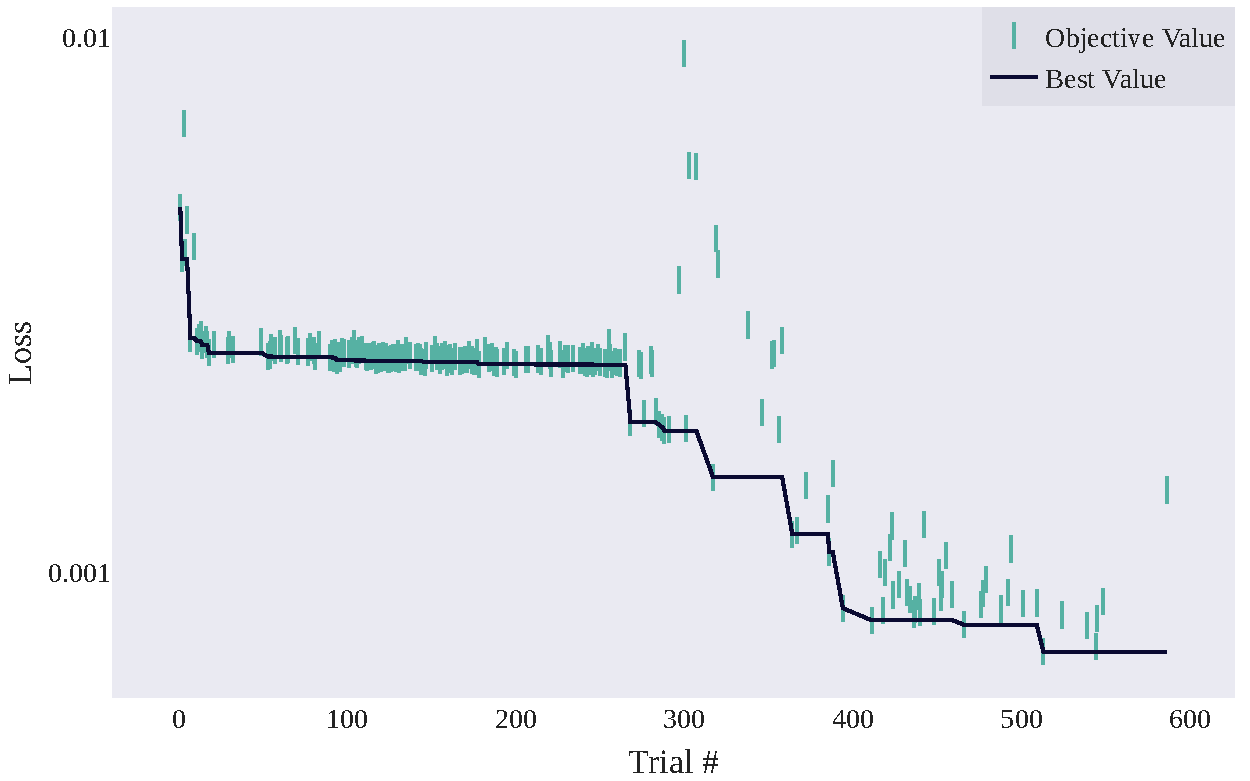
\includegraphics[width=12cm,height=7cm]{images/chapter_3/Optimization_History.pdf}
\caption{Best loss values found during hyper-parameter optimization. The effect of a switch to random sampling and an increase of the pruning threshold can be observed during trials 270 and 310.}
\label{chap3:bestvalues}
\end{figure}

\begin{figure}[htbp]
\centering
\textbf{Loss Value per Epoch for Top 10 Trials}
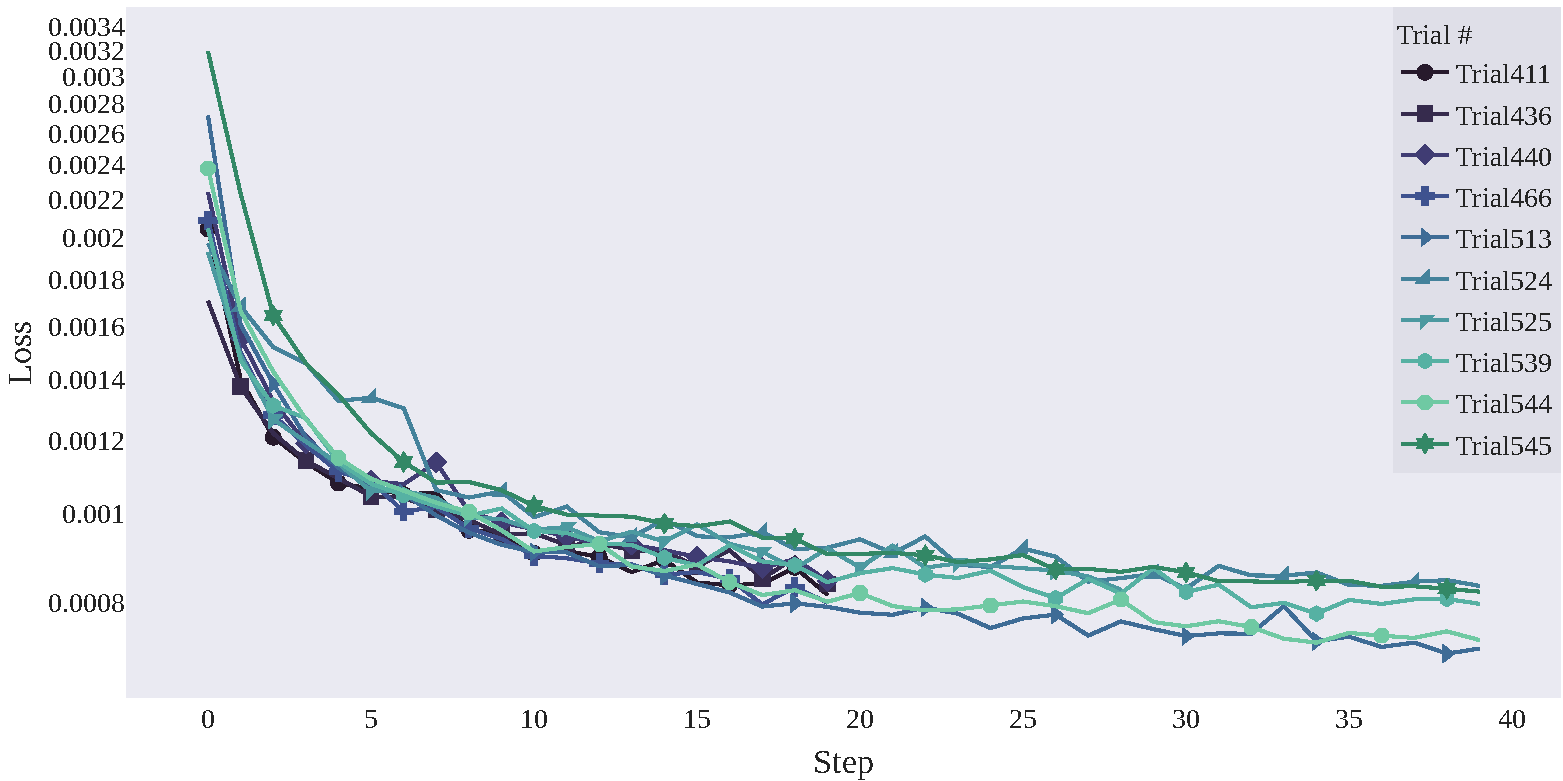
\includegraphics[width=12cm,height=6.5cm]{images/chapter_3/loss_per_training.pdf}
\caption{Loss value per epoch for top 10 trials. Some of the initial 500 trials appear in this list, despite having half the number of epoch steps. The learning curves tend to flatten quickly. Therefore, 20 epoch steps may be a reasonable number for measuring hyper-parameter viability. }
\label{chap3:top10}
\end{figure}


\begin{figure}[t]
\begin{center}
    \textbf{Hyper-Parameters' Loss Correlation}
    \makebox[\textwidth]{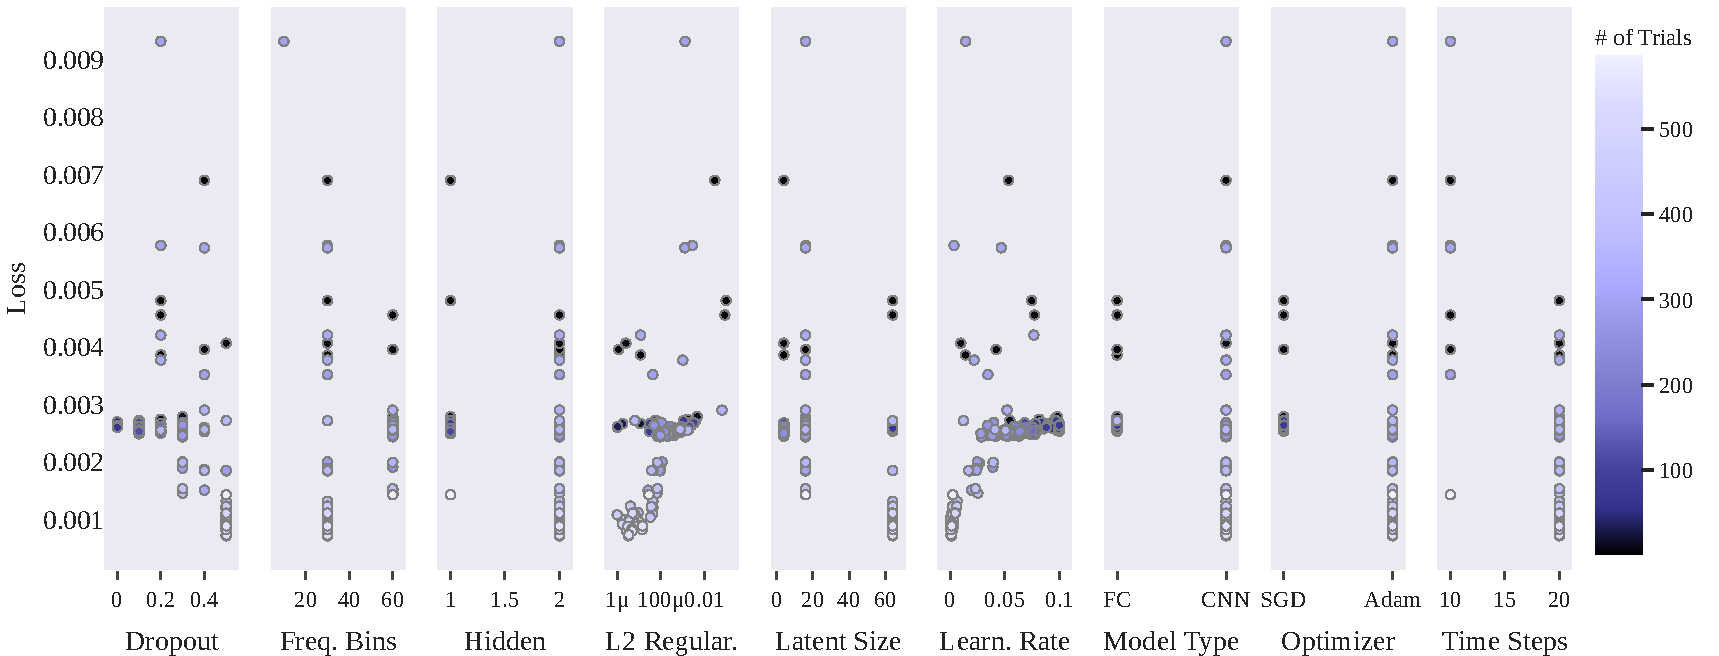
\includegraphics[width=0.95\paperwidth]{images/chapter_3/slice_plot.pdf}}
      \caption{Sliced plot depicting the correlation between hyper-parameters and loss values. The color-scale shows the number of times each parameters has been used in a trial. Our sampling algorithm aims to utilize spaces with higher potential more often. }
    \label{fig:slicegraph}
    \end{center}

\end{figure}
\begin{figure}[h!]
\begin{center}
    \textbf{ Parallel Coordinates of Hyper-Parameter Sets and Loss}
    \makebox[\textwidth]{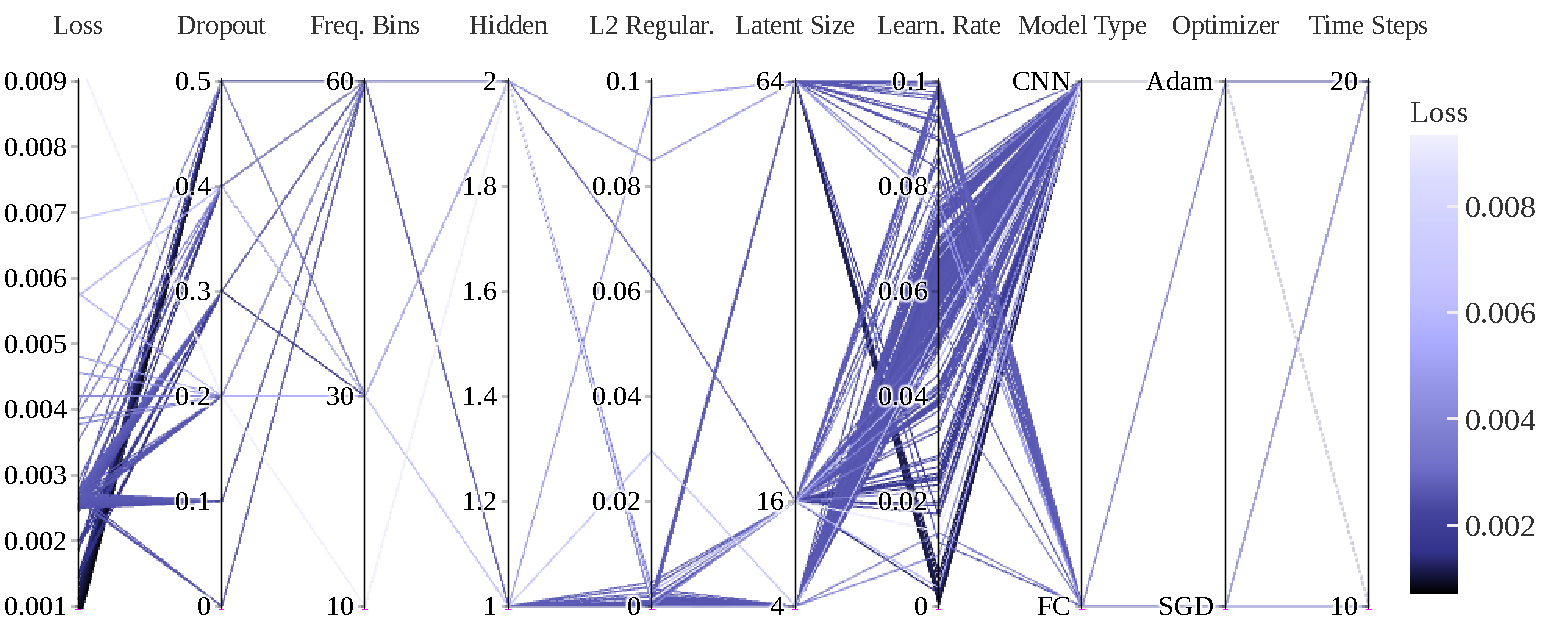
\includegraphics[width=0.9\paperwidth]{images/chapter_3/parallel_coord.pdf}}
      \caption{Not sure if worth keeping. Paths connect hyper-parameters in a set. Path's are colored based on loss value.}
       \label{fig:parallel_coord}
    \end{center}
   
\end{figure}

We depict the correlation of parameter values with trial results in figures~\ref{fig:slicegraph} and~\ref{fig:parallel_coord}. We extract a more concrete measurement of hyper-parameter influence using Hutter et al.'s fANOVA importance evaluator~\cite{hutter2014efficient}. We limit this analysis to 500 trials with 20 epochs. The results of this estimation are depicted in figure~\ref{chap3:param_importance}. Contrasting the results of the fANOVA evaluator with figure~\ref{fig:slicegraph}, we notice several issues. Notably, the importance of 0 is attributed to "Model Type" and "Optimizer" parameters, despite a visible difference depicted in the slice-graph. This may be due to the imbalanced sampling of the hyper-parameter space, prompted by our greedy search in place of random sampling. Another possible cause is the "averaging" of loss results regardless of variance: For example, the slice-graph depicts CNN models as having the best and worst results while FC models are reliably average; Making the fANOVA's 0 importance attribution logical, but not optimal when we are strictly looking for the best models. 

\begin{figure}[t!]
\centering
\textbf{Estimated Parameter Importance}
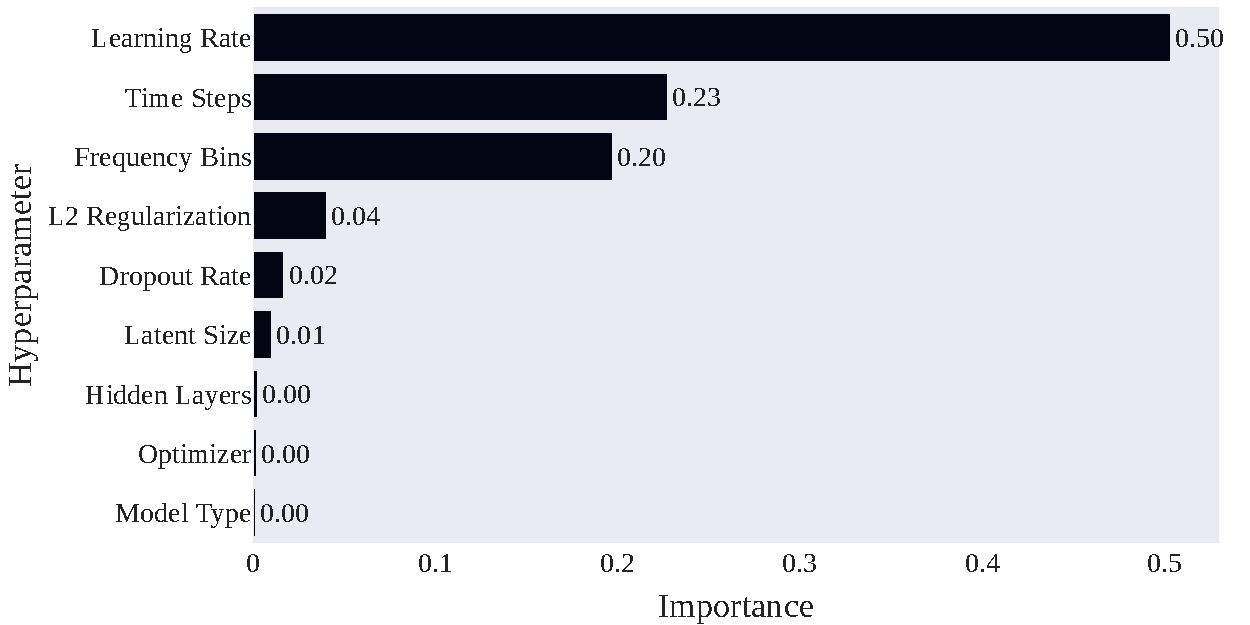
\includegraphics[width=14cm,height=7cm]{images/chapter_3/ParameterImportances_final.pdf}
\caption{The parameters' estimated importance in determining the outcome of trials. Specifications of the spectrogram seem to affect the outcome more so than the model's configuration. We attribute the contrast between the results here and those in figure~\ref{fig:slicegraph} and~\ref{fig:parallel_coord} to the irregular rate of sampling from the hyper-parameter space.}
\label{chap3:param_importance}
\end{figure}

\subsubsection{Possible Explanation for Embedding Ear's Effectiveness}
How well does our best autoencoder work? What happens if we create a feedback loop where a decoded spectrograms are fed through the network again? 
\begin{figure}[h!]
\centering
\textbf{Recursive Recreation of Drums and Synthetic Noise}\par\medskip
\makebox[\linewidth][c]{%
\begin{subfigure}[b]{.6\textwidth}
\centering
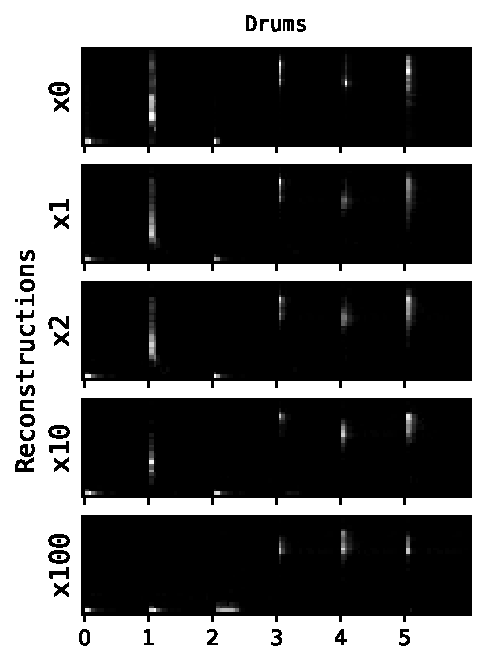
\includegraphics[width=.95\textwidth]{images/chapter_3/Drums_reacreation.pdf}
% \caption{a test subfigure}
\end{subfigure}%
\begin{subfigure}[b]{.6\textwidth}
\centering
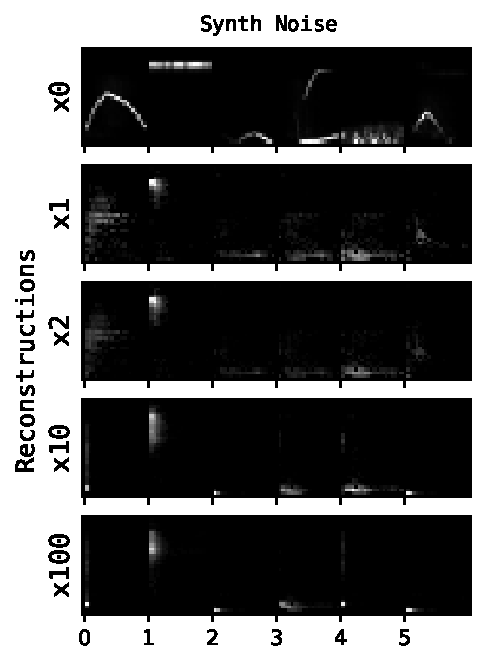
\includegraphics[width=.95\textwidth]{images/chapter_3/Synth Noise_reacreation.pdf}
% \caption{a test subfigure}
\end{subfigure}%
}\\
\caption{We concatenate 6 spectrograms for drum and synthetic noise groups. We recursively encode and decode these spectrograms and display the results. The first row depicts the unaltered spectrograms. We display the results after 1, 2, 10 and 100 recursive recreations. We see that drum spectrograms retain their original form better than synthetic noise.}
\label{fig:recreations}
\end{figure}

We recursively run the autoencoder on new sounds and display the results in figure ~\ref{fig:recreations}. The results are displayed for 1, 2, 10 and 100 recursions. Spectrograms belonging to percussive groups retain their unique characteristics for a few time steps, while details in most synthetic noise spectrograms are quickly dissipated. A major point of concern here is that recursively recreated synthetic noise spectrograms tend to take on drum characteristics. This is possibly prompted by our encoder only having been exposed to drums sounds prior.  Yet it is possible that the "confusion" demonstrated by the encoder after the initial reconstruction leads to embedding of familiar sounds being distinguishable from those unseen. If correct, this approach may have beneficial implications in addressing the aforementioned OSR problem.  


\subsubsection{Feature Extraction}
\label{fig:embedding_FE}
\begin{table}[htbp!]
\centering
\begin{tabular}{|p{6cm}|p{6cm}|}
\hline
Hyper-Param. & Value  \\ \hline
Model Type      &  CNN  \\ \hline
Optimizer       & Adam  \\ \hline
Hidden Layers   & -  \\\hline
Learning Rate   &  0.001145\\ \hline
Frequency Bins & 30 \\ \hline
Time Steps & 20 \\ \hline
Latent Size & 64 \\ \hline
Regularization & 3.25^{-6}\\ \hline
Dropout Rate & 0.5 \\ \hline
\end{tabular}
\caption{Top performing hyper-parameter set}
\label{table:best_params}
\end{table}
\begin{figure}[h!]
\centering
\textbf{2 Dimensional Projection of Latent Variables}\par\medskip
 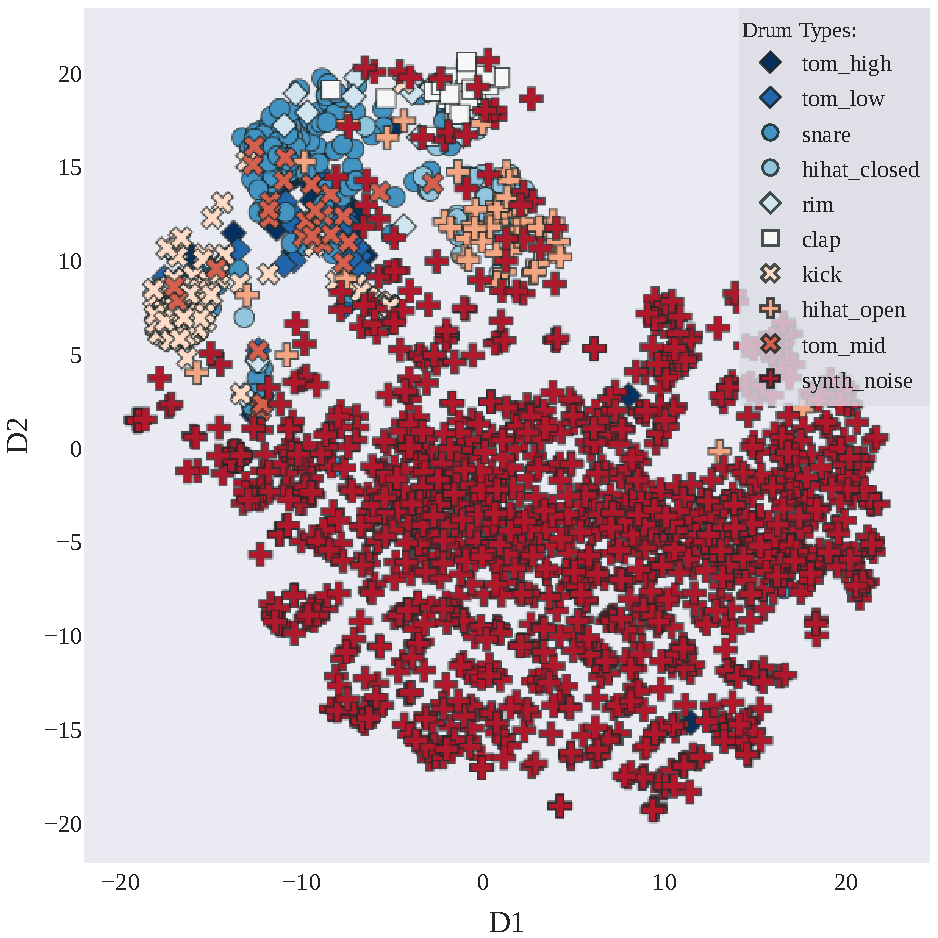
\includegraphics[width=0.90\linewidth]{images/chapter_3/t-SNE_2d.pdf}
\caption{Projection of an embedding model's low dimensional encoding on to a 2D plane. We implemented interactions for these graphs for manual inspection of samples.}
\label{fig:2d_tsne}
\end{figure}

\begin{figure}[htbp!]
\centering
\textbf{3D t-SNE Projection}\par\medskip
\mbox{\subfloat[]{\label{subfig:1} \fbox{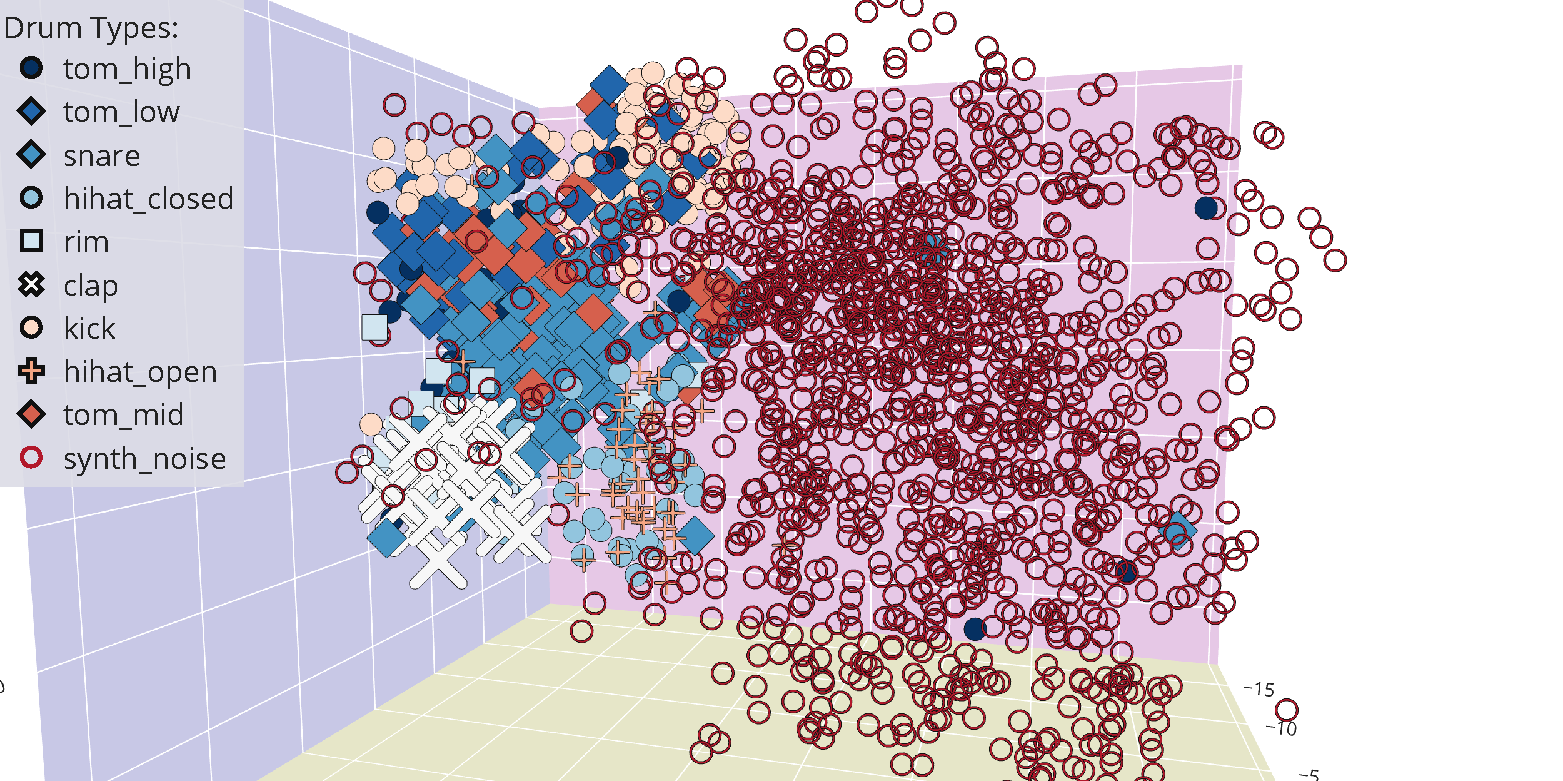
\includegraphics[width=14cm,height=6.8cm]{images/chapter_3/3d_t-SNE_symdrum_type_cam0.pdf}}}}

\mbox{\subfloat[]{\label{subfig:2} \fbox{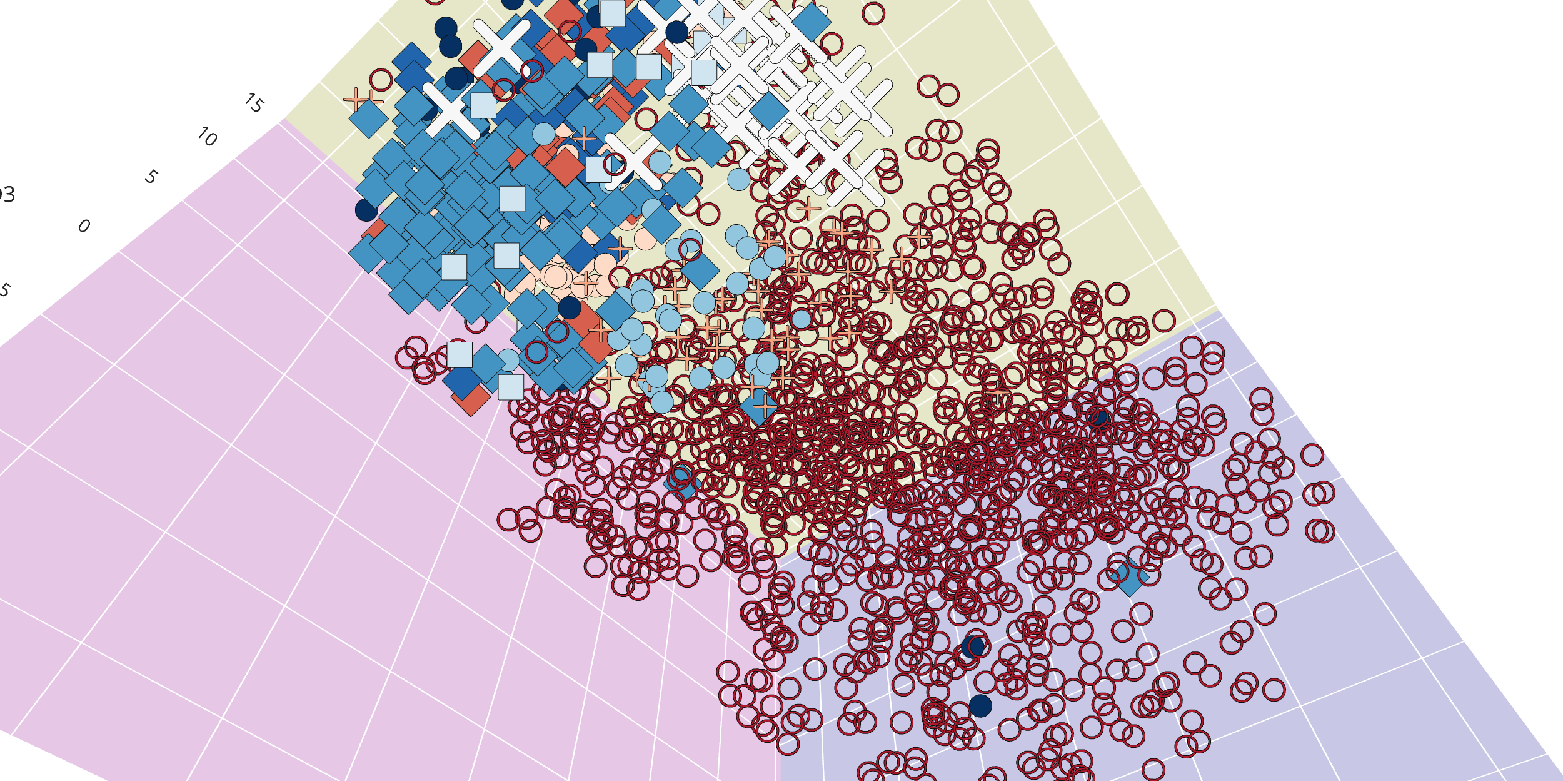
\includegraphics[width=14cm,height=6.8cm]{images/chapter_3/3d_t-SNE_symdrum_type_cam3.pdf}}}}

\fbox{\mbox{\subfloat[]{\label{subfig:2} 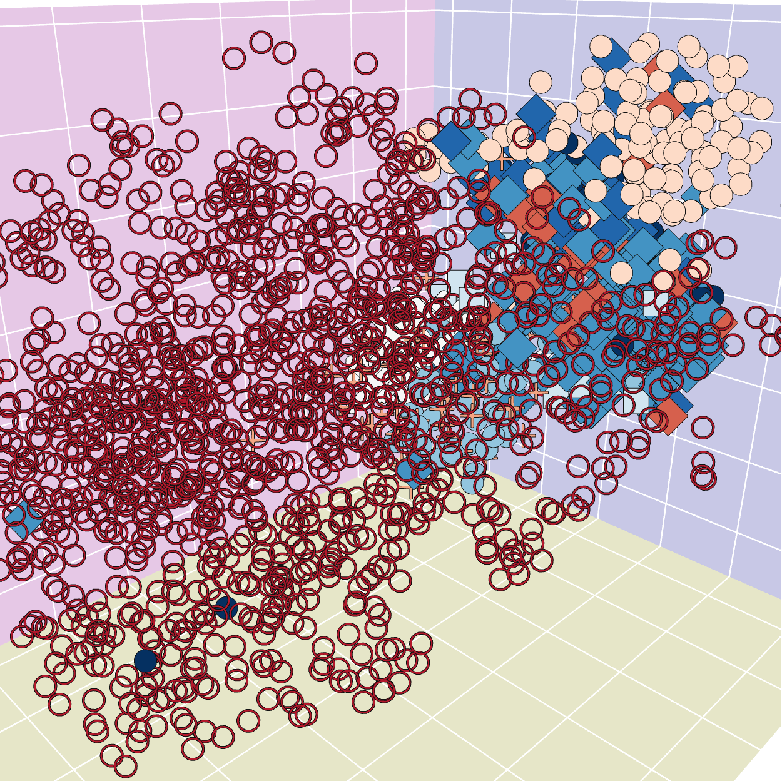
\includegraphics[width=5cm,height=5cm]{images/chapter_3/3d_t-SNE_symdrum_type_cam1.pdf}}}
\mbox{\subfloat[]{\label{subfig:2} 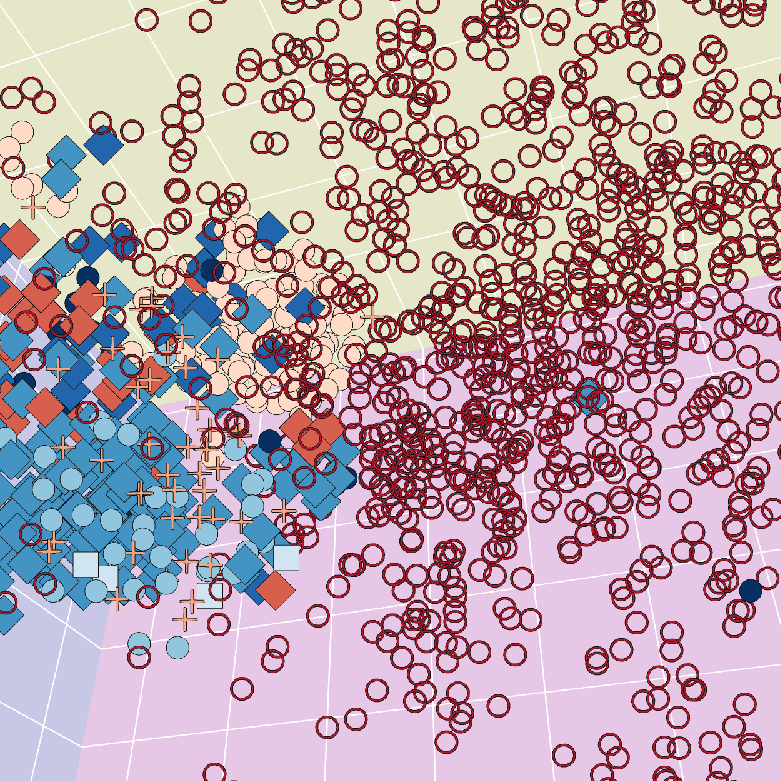
\includegraphics[width=5cm,height=5cm]{images/chapter_3/3d_t-SNE_symdrum_type_cam2.pdf}}}}
\caption{Our feature projections and interactive graphs can also be done in 3D}
\label{fig:3d_tsne}
\end{figure}
To better understand the delineation potential of the encoded features,  we trained an autoencoder with our top performing hyper-parameter set, shown in table ~\ref{table:best_params}. We used \%80 of MixedDB to train the model for 200 epochs. Using this model, we encoded the remaining \%20 and approximately 1000 randomly selected sounds from NoiseDB into 64 dimensions. These 64-dimensions were then projected onto a 2 or 3-dimensional plane using t-SNE. Referring to~\hypref{Decision.1} and~\hypref{Decision.2} to define our expectation of a useful encoder, we expect the drum sounds to be clustered together, with the majority of the synthetic noise sounds appearing away from these clusters. Our projections confirm that this is the case. We are most interested in synthetic noise sounds which appear within or near these clusters. Do these synthetic noise sounds have drum like characteristics?\\ 


To test this, we implemented interactive graphs identical to those depicted in figures \ref{fig:2d_tsne} and~\ref{fig:3d_tsne}; Interactive graphs allow interactions such as playing the samples(by hovering the cursor on-top) and movement of the scene camera.  Manual inspection reveals a noticeable, positive correlation between distance and similarity of a synthetic sound to a drum cluster. Divergences from the envelope features expected from drums are a common point of failure. A noticeable case was a synthetic noise resembeling a \emph{reverse} kick drum within the kick cluster. While encouraging, we hypothesize that more specialized forms of encoding or addition of other features are needed for reducing the frequency of errors and strengthening this correlation.

We see possible benefits in a mixture of envelope features with embedding features. In section~\ref{chap3:mixed_ear_models}, we analyze the potential gains in using both features for extraction of drum-like sounds from synthetic noise. 

\subsection{Mixed Ear Models}
\label{chap3:mixed_ear_models}
As t-SNE results are not classifiers in of themselves, we create a model which uses encoded versions of each sound group to predict its type. This differs from two-phased ears as we are simultaneously categorizing a new sound's drum type or putting it in the "synthetic noise" category. We call this task drum vs drum vs not-drum, or "DvDvN". We also tackle the Drum vs Not-Drum problem using our embedding features.

As discussed in Section \label{fig:embedding_FE}, manual t-SNE inspections highlighted the disregard for envelope shapes as a major source of failure. We compare the performance of our models before and after the addition of envelope features (a vector of size 10) to the feature space. 

We reuse the model trained on  MixedDB as our embedding feature extractor. We use a combination of RadarDB, FreeDB and NoiseDB for training. We only focus on clap,hat,kick,snares, synthetic noise groups for measuring effectiveness to prevent class overlaps as much as possible. We also exclude samples longer than 1 second, to exclude potentially mislabeled data. Our final training database for mixed ear models is described in table~\ref{db:memDB}.

\subsubsection{Model Selection}
Using our encoding and envelope features to represent audio, five classification models were trained for the task of categorizing the five different sound groups. For hyper-parameter optimization, the models were trained using 5-fold cross validation and 80/20 train-to-test ratio. The F-Score result of each cross-validation is the unweighted average F-Score of all groups. For inter-model comparisons, the procedure is the same except 10-fold cross validations are used. Our models were derived from scikit-learn's implementations of these classifiers~\cite{pedregosa2011scikit}. Before inter-model comparisons, we conducted a grid-search for each model on at least one of its possibly decisive hyper-parameters. The classifiers and other notable specifications are presented in table~\ref{table:mem_model_selection}. We introduced class weights where possible to mitigate the effects of an imbalanced dataset~\cite{provost2000machine,chawla2004special}. When utilized, the weight for each class $c$  is calculated as:

\begin{subequations}
    \begin{align*}
    c_{weight} = 1-\dfrac{\text{number of samples in group $c$} }{\text{Total number of samples}}
    \end{align*}
\end{subequations}

\begin{table}[t]
    \centering \hspace*{-0.8cm}
    \begin{threeparttable}
    \begin{tabular}[width=0.95\paperwidth]{|l|l|l|}
    \hline
    Model name & Tuned Parameters\tnote{\dag}  & Used Weights? \tnote{\ddag} \\\hline
     Support Vector Classifier (SVC) &  Gamma:0.001, C:100, kernel:rbf & Yes\\
     LinearSVC & C:10 & Yes\\
     K Nearest Neighbors & Num. Neighbors:30 &  No \\
     Random Forest Classifier & Num Estimators:500 & Yes \\
     Extra Trees Classifier & Num Estimators:1100 & Yes\\
     \hline
    \end{tabular}
    \caption{Models implemented for comparison using envelope and embedded features. }
    \begin{tablenotes}
    \item[\dag] Tuned parameters values are based on grid-searching for best f-score. Parameters not mentioned have neither been tuned nor changed from scikit-learn's default values (as of version 0.23)
    \item[\ddag] Class weights are used unless not applicable to classifier.
    \end{tablenotes}
    \label{table:mem_model_selection}
    \end{threeparttable}
\end{table}
\begin{table}[hp!]
\centering
\begin{tabular}{|l|l|l|l|l|l|}
\hline
 DB Name & kick & snare & clap & hat & Synthetic Noise\\\hline
 MixedEarDB & 1334 & 1035 & 401 & 1275 & 1000 \\ \hline
\end{tabular}
\caption{MixedEarDB: A database put together by combination of radarDB, FreeDB and NoiseDB}
\label{db:memDB}
\end{table}

\begin{figure}[htbp!]
    \begin{center}
    \textbf{Cross Validation F-Scores For All Sound Groups}\par\medskip
    \makebox[\textwidth]{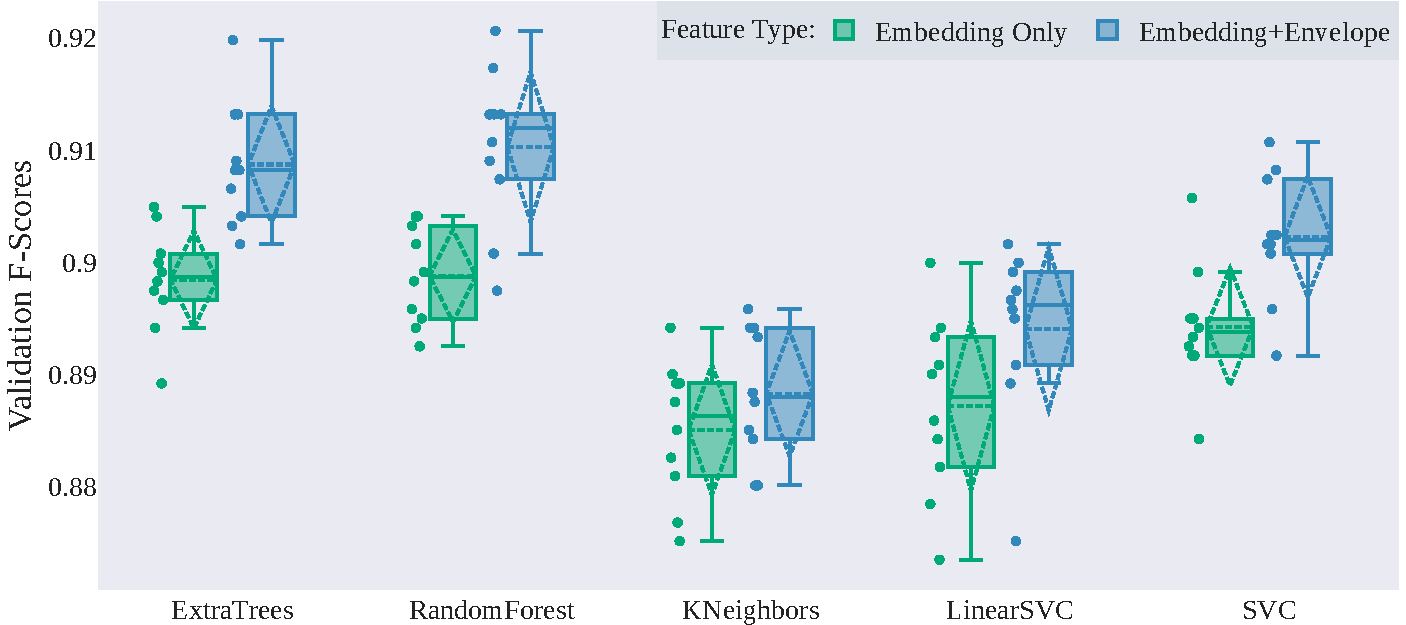
\includegraphics[width=0.8\paperwidth]{images/chapter_3/mme_comparisons_mme.pdf}}
    \caption{Boxplots visualizing the F-Score results for each cross-validation. The individual scores, means, medians, standard-deviation and outliers are depicted. The differences are noticeable, yet means lie within the \%88-92 range. Envelope features improve classification accuracy for all models. }
    \label{fig:f1_allg_box}
    \end{center}

\end{figure}


We're also interested in how these models perform on the binary drum vs not drum task.
After grouping all drums together, we repeat the model selection process above. We also repeat the hyper-parameter optimization step where no changes appeared necessary except for a reduction in the number of neighbors for the K-Neighbor model (from 30 to 5). As show in in figures~\ref{fig:f1_allg_box} and~\ref{fig:f1_dvn_box}, the addition of envelope features had a positive effect on performance for all mdoels, yet the RandomForest and ExtraTrees models clearly outperform the other classifiers in both tasks. We train the top two models on \%80 of our database and use the remaining \%20 to create the confusion matrices and the F-Scores shown in figures~\ref{fig:conf_f1}.


\begin{figure}[h!]   

    \begin{center}
        \textbf{Cross Validation F-Scores For Drum Vs Not-Drum}
    \makebox[\textwidth]{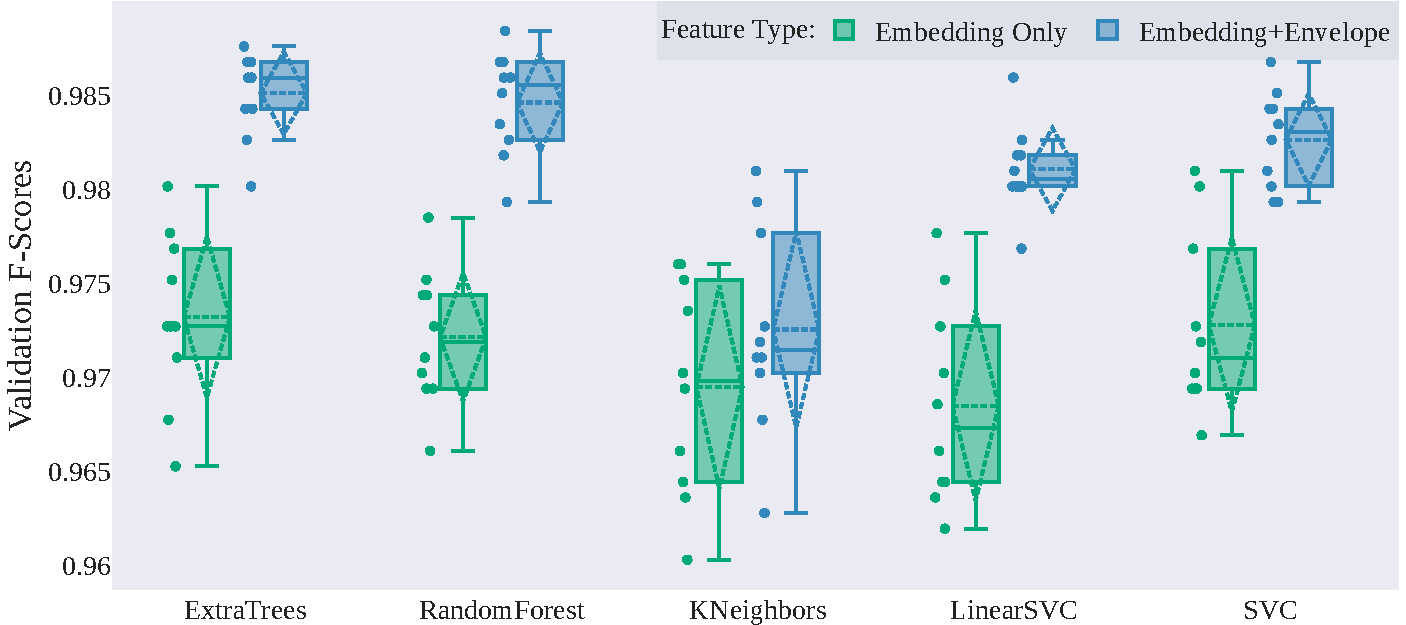
\includegraphics[width=0.8\paperwidth]{images/chapter_3/mme_comparisons_dvn.pdf}}
    \caption{F-Score results for each cross-validation. Models perform better as there are less categorization groups. Envelope features increase accuracy for all models. Random Forest and Extra Trees remain the top two models. }
    \label{fig:f1_dvn_box}
    \end{center}

\end{figure}


\begin{figure}[htbp!]
\begin{center}
    \textbf{Classification Report of Best Performing Model}\par\medskip
    \makebox[\textwidth]{
    \subfloat[Precision, recall, F1-Score, and number of supporting examples]{ 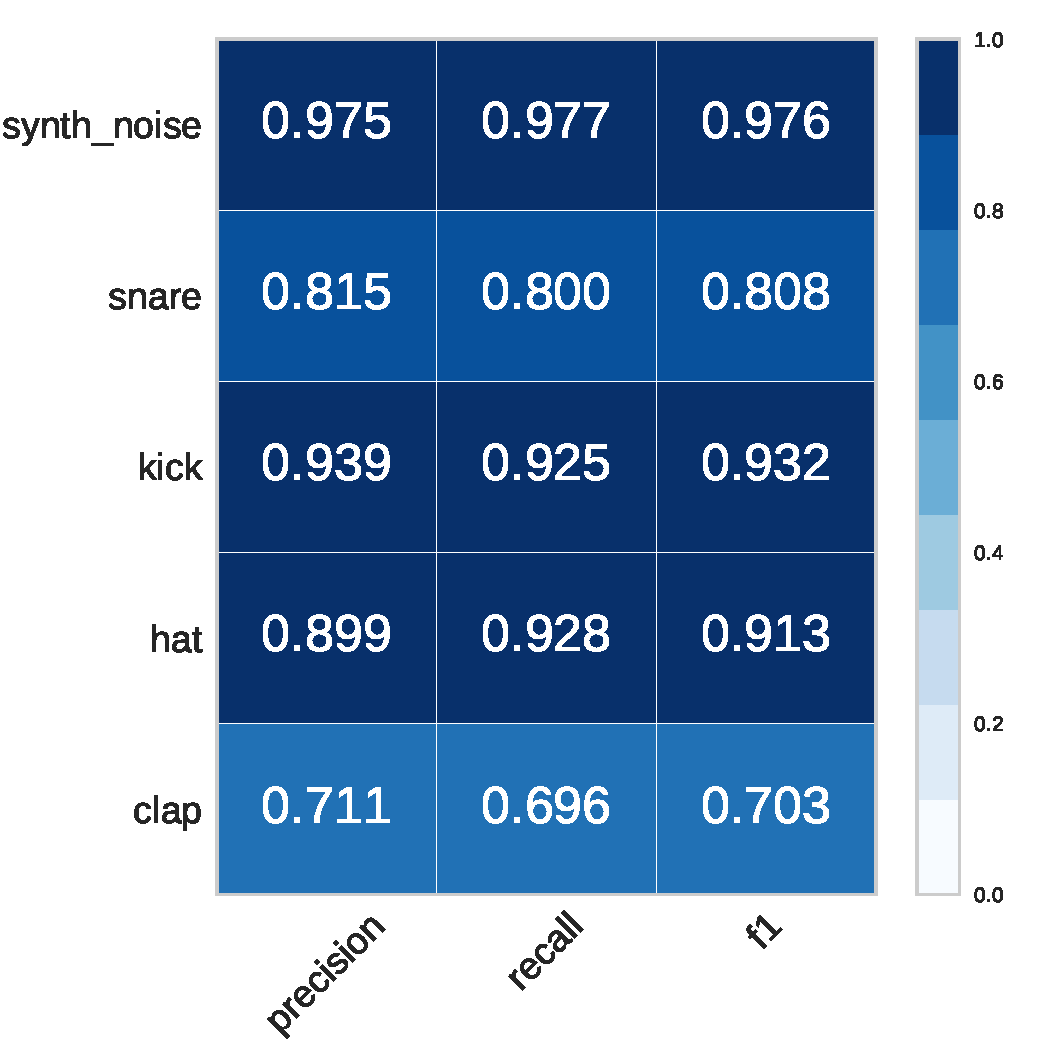
\includegraphics[width=9cm,height=9cm]{images/chapter_3/f1_mme.pdf}
    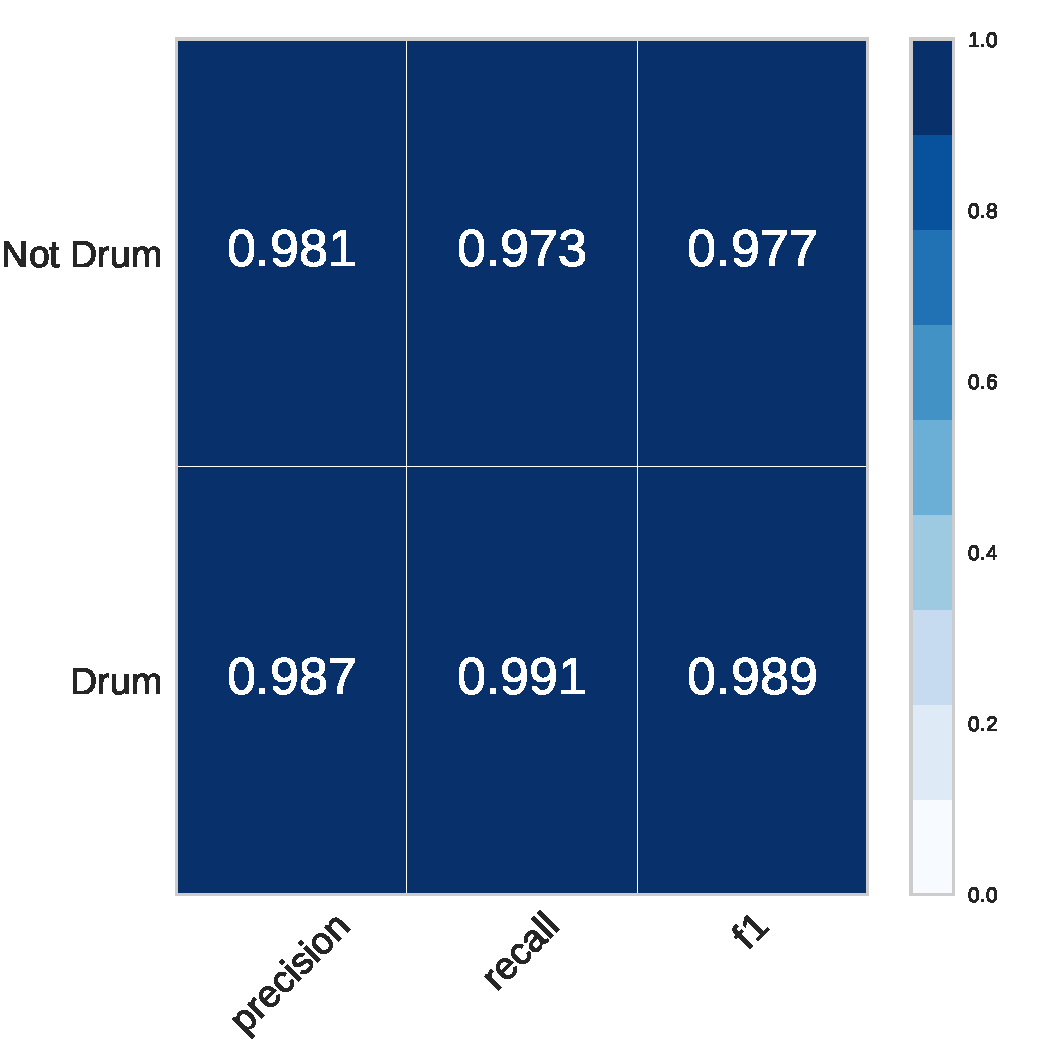
\includegraphics[width=9cm,height=9cm]{images/chapter_3/f1_dvn.pdf}
    }
    
    }
    
\end{center}

\begin{center}
    \makebox[\textwidth]{
    \subfloat[Confusion matrices for both tasks]{ 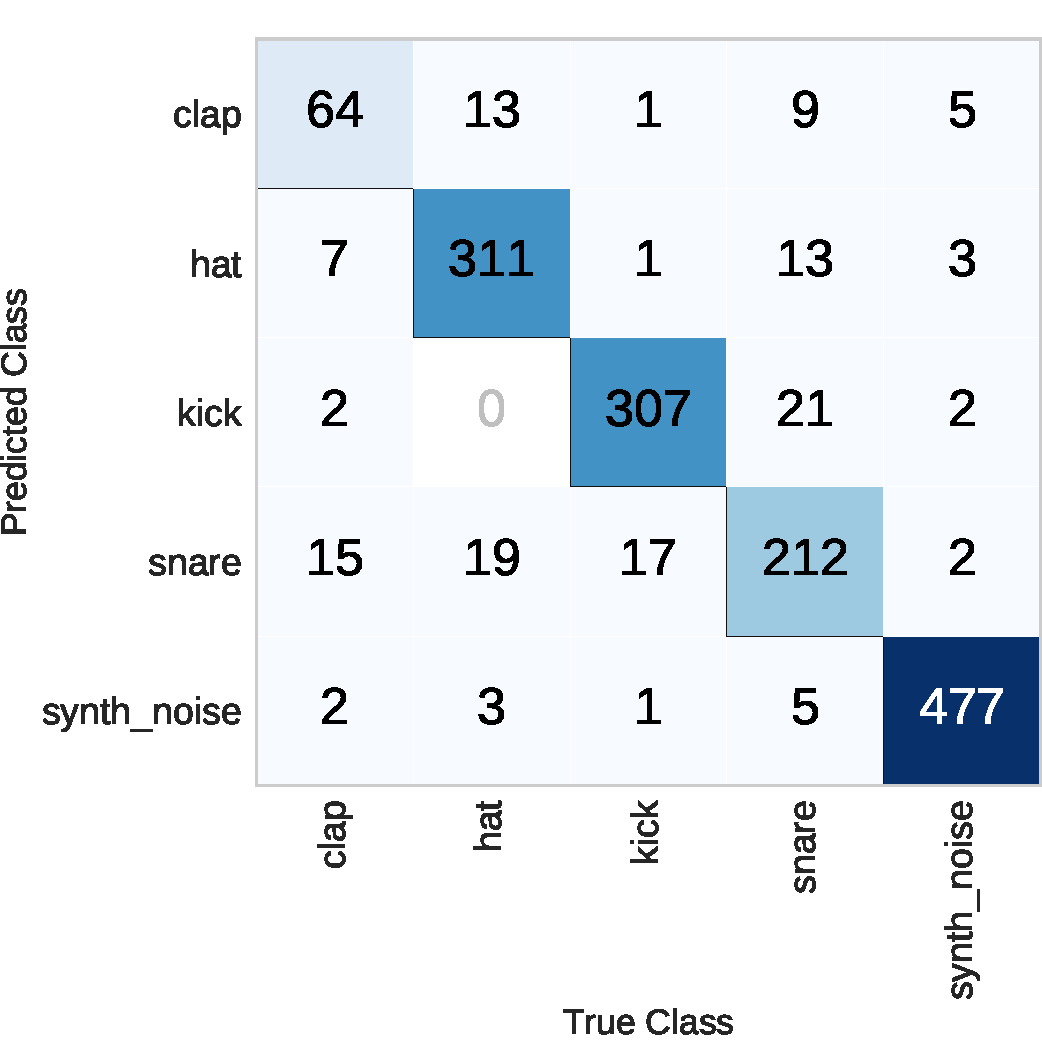
\includegraphics[width=9cm,height=9cm]{images/chapter_3/conf_mme.pdf}
    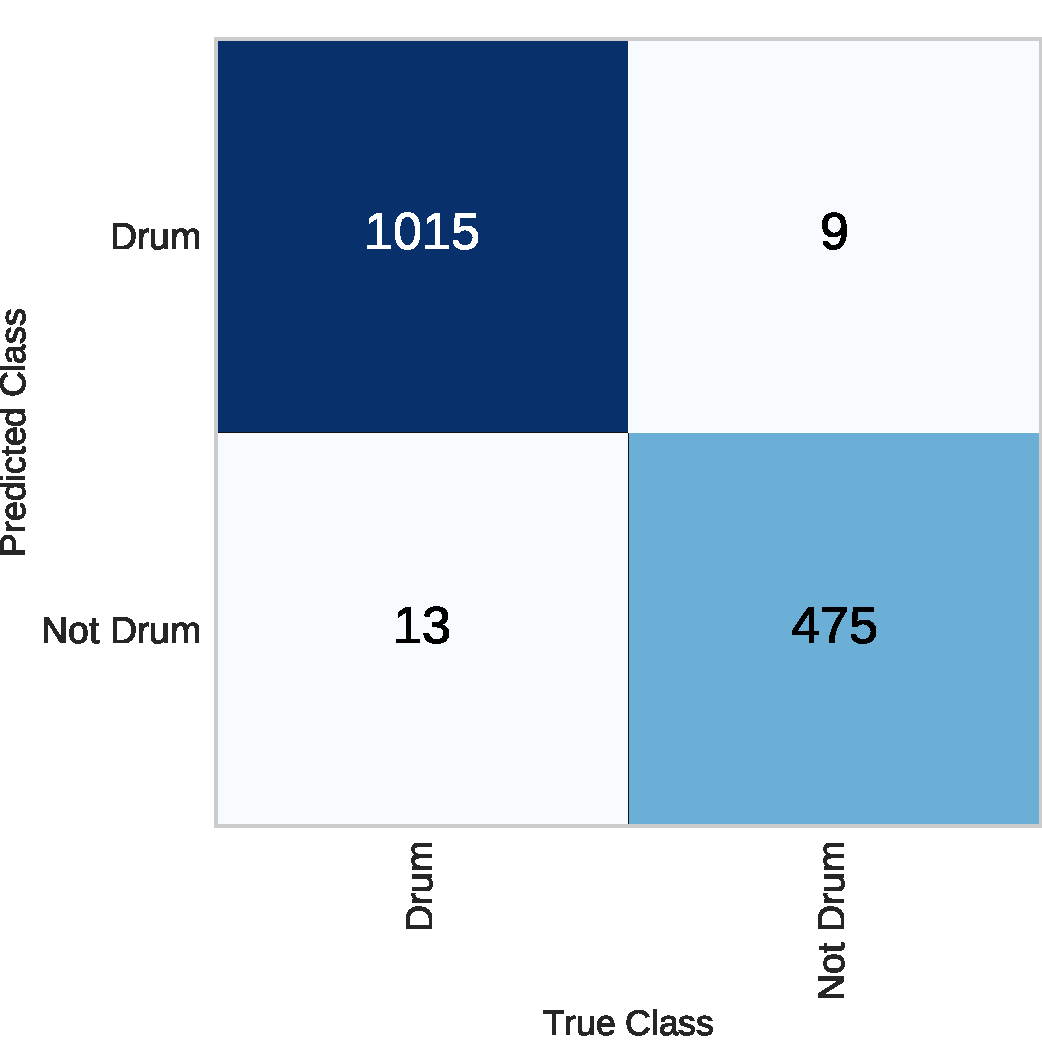
\includegraphics[width=9cm,height=9cm]{images/chapter_3/conf_dvn.pdf}
    }}
\end{center}


\caption{F-Scores and confusion matrix of ExtraTrees model for both DvDvN and drum vs not-drum categorization.}
\label{fig:conf_f1}
\end{figure}

Based on these reports, having multiple options for drum categorization does not noticeably influence our models accuracy in categorizing synthetic noise as synthetic noise. However, the DvDvN models's slightly smaller false negative rate for synthetic noise (11 vs 13 false negatives) is countered by a slightly higher rate of categorizing drums as synthetic noise (12 vs 9).  We therefore use the DvDvN implementation as it simultaneously categorizes drum types and separates noise from drums. However, without manual insepction, we cannot confirm the extend of this model's usefulness. 

We create the mixed ear model by combining our encoder with the ExtraTrees classifier. As sounds are generated with the virtual synthesizer, the encoding and envelope features will be extracted using the encoder and sent to the ExtraTrees DvDvN classifier. In the upcoming novel generations section, we will present the results of a two person survey where the accuracy of the two-ear model is analyzed given 500 synthetic noise sounds categorized as drums. 



\section{Data And Project Replication}

Our data sources are a large set of 2 second or shorter drum samples aggregated from personal libraries, free drum kits from the sample-swap project \footnote{https://sampleswap.org/} which we organized into 5 groups, and a large set of drum sounds aggregated from royalty free sources such as musicradar \footnote{https://www.musicradar.com/}. We put together 3 databases of drums using these sources. We also created a database of synthetic noise from 1, 3, and 5 stacked virtual synthesizers. Specifications about our datasets can be found in tables~\ref{db:self},~\ref{db:radar}, ~\ref{db:sampleswap} and ~\ref{db:noise}. We have made our dataset of free-drum sounds available for download. The scripts used to download and process royalty free samples are also made available. Further information about downloading our dataset can be found on the project's github page. 

We prioritize making generalizable tools which can learn from and produce a variety of different sounds. We utilize these databases depending on the task at hand. At times, we merged or purged drum groups to simplify tasks. The "merge-able" groups are specified in table~\ref{db:merge-map}. Where relevant, we will specify which databases have been used and whether any merging or purging of sound groups has taken place. 

% \begin{itemize}
% \item The kick, snare and hat categories have the largest share at around 20\% each, while the shaker and rim (other) categories have the smallest at 5\% combined. Due to this we only focused on learning from kicks, snares, toms, claps and hats for Phase 1 of training (along with non-percussive groups of sound) ~\ref{sec:ear}.

% \item For Phase 2 of training we only focused on categorizing snares, claps, kicks, hats and other (percussive sounds such as shakers, rims and unusual percussions that we couldn't categorize were grouped into this category). Non-percussive datasets were not used for this phase. 
% \item In order to offset bias from data imbalance during training of our models, the categorical cross entropy loss was weighted by the group sizes. 
% \item For any given model, 80\% of our data is used for training and 20\% is used for testing. 

% \item We limit the size of the n-stack-synths category to 50\% of the total size of our drum dataset. This is done in order to measure whether the features extracted can address the "Open Set Recognition" problem, which will be discussed further in Section ~\ref{sec:ear}.
% \end{itemize}

\begin{table}[p]
\centering
\hspace*{-2cm}\begin{tabular}[width=0.95\paperwidth]{|l|l|l|l|l|l|l|l|l|l|}
\hline
DB Name & kick & snare & clap & tom\_high & tom\_mid & tom\_low & hihat\_closed &  hihat\_open & rim \\ \hline
MixedDB & 648 & 732 & 118 & 179 & 139 &  188 & 187 & 280 & 105 \\\hline
\end{tabular}
\caption{Database 1: Mixed sources}
\label{db:self}
\end{table}

\begin{table}[h!]
\centering
\begin{tabular}{|l|l|l|l|l|l|l|l|l|}
\hline
DB Name & kick & snare & clap & tom & clap & hat & rim & shaker  \\ \hline
RadarDB & 1054 & 842   & 353 & 349 &  353 & 1561& 131 & 121 \\ \hline
\end{tabular}
\caption{Database 2: Royalty free sounds sourced from "Music Radar"}
\label{db:radar}
\end{table}

\begin{table}[h!]
\centering
\begin{tabular}{|l|l|l|l|l|l|}
\hline
 DB Name & kick & snare & clap & hat & other \\\hline
 FreeDB & 533 & 372 & 230 & 105 & 281 \\ \hline
\end{tabular}
\caption{Database 3: Free sounds sourced from the "Sample Swap" project. Simplified for our purposes. The version available for download contains more sample groups. The "other" category contains a variety of percussive sounds.}
\label{db:sampleswap}
\end{table}


\begin{table}[h!]
\centering
\begin{tabular}{|l|lll|}
\hline
 Synth Noise Type &1 Stack & 3 Stacks  & 5 Stacks \\ \hline
 Number of Examples &2000 & 2000 & 2000 & \hline
\end{tabular}
\caption{Database of random noise examples from our virtual synthesizers}
\label{db:noise}
\end{table}

\begin{table}[h!]
\centering
\begin{tabular}{|p{3cm}|p{8cm}|}
\hline
 Merged Name & Possible Merged Groups \\ \hline
 Kicks & low toms and kicks \\
 Toms & toms and mid toms \\
 Snares & snares and high toms  \\
 Hats & high hats and low hats \\ 
 Other & rims, shakers and other percussive sounds with few representative samples \\ \hline
\end{tabular}
\caption{These mappings may be used to simplify databases. }
\label{db:merge_map}
\end{table}

\end{document}